%%%%%%%%%%%%%%%%%%%%%%%%%%%%%%%%%%%%%%%%%
% Masters/Doctoral Thesis 
% LaTeX Template
% Version 2.4 (22/11/16)
%
% This template has been downloaded from:
% http://www.LaTeXTemplates.com
%
% Version 2.x major modifications by:
% Vel (vel@latextemplates.com)
%
% This template is based on a template by:
% Steve Gunn (http://users.ecs.soton.ac.uk/srg/softwaretools/document/templates/)
% Sunil Patel (http://www.sunilpatel.co.uk/thesis-template/)
%
% Template license:
% CC BY-NC-SA 3.0 (http://creativecommons.org/licenses/by-nc-sa/3.0/)
%
%%%%%%%%%%%%%%%%%%%%%%%%%%%%%%%%%%%%%%%%%

%----------------------------------------------------------------------------------------
%	PACKAGES AND OTHER DOCUMENT CONFIGURATIONS
%----------------------------------------------------------------------------------------

\documentclass[
11pt, % The default document font size, options: 10pt, 11pt, 12pt
%oneside, % Two side (alternating margins) for binding by default, uncomment to switch to one side
english, % ngerman for German
singlespacing, % Single line spacing, alternatives: onehalfspacing or doublespacing
%draft, % Uncomment to enable draft mode (no pictures, no links, overfull hboxes indicated)
%nolistspacing, % If the document is onehalfspacing or doublespacing, uncomment this to set spacing in lists to single
%liststotoc, % Uncomment to add the list of figures/tables/etc to the table of contents
%toctotoc, % Uncomment to add the main table of contents to the table of contents
%parskip, % Uncomment to add space between paragraphs
nohyperref, % Uncomment to not load the hyperref package
headsepline, % Uncomment to get a line under the header
%chapterinoneline, % Uncomment to place the chapter title next to the number on one line
%consistentlayout, % Uncomment to change the layout of the declaration, abstract and acknowledgements pages to match the default layout
]{MastersDoctoralThesis} % The class file specifying the document structure

\usepackage[utf8]{inputenc} % Required for inputting international characters
\usepackage[T1]{fontenc} % Output font encoding for international characters

\usepackage{palatino} % Use the Palatino font by default

\usepackage[dvipdfmx]{hyperref}
\hypersetup{pdfpagemode={UseOutlines},
bookmarksopen=true,colorlinks=true,citecolor=blue,linkcolor=blue,urlcolor=blue}

%\usepackage[backend=bibtex,style=authoryear,natbib=true]{biblatex} % Use the bibtex backend with the authoryear citation style (which resembles APA)

\usepackage[backend=bibtex,style=phys,natbib=true]{biblatex}
\addbibresource{pcal.bib}
%\AtEveryBibitem{\clearfield{title}}
%\AtEveryBibitem{\clearfield{doi}}
%\AtEveryBibitem{\clearfield{eprint}}

\usepackage[autostyle=true]{csquotes} % Required to generate language-dependent quotes in the bibliography

%----------------------------------------------------------------------------------------
%	MARGIN SETTINGS
%----------------------------------------------------------------------------------------

\geometry{
	paper=a4paper, % Change to letterpaper for US letter
	inner=2.5cm, % Inner margin
	outer=3.8cm, % Outer margin
	bindingoffset=.5cm, % Binding offset
	top=1.5cm, % Top margin
	bottom=1.5cm, % Bottom margin
	%showframe, % Uncomment to show how the type block is set on the page
}

%----------------------------------------------------------------------------------------
%	THESIS INFORMATION
%----------------------------------------------------------------------------------------

\thesistitle{KAGRA photon calibrator} % Your thesis title, this is used in the title and abstract, print it elsewhere with \ttitle
\supervisor{Prof. Rick \textsc{Savage}} % Your supervisor's name, this is used in the title page, print it elsewhere with \supname
\examiner{} % Your examiner's name, this is not currently used anywhere in the template, print it elsewhere with \examname
\degree{} % Your degree name, this is used in the title page and abstract, print it elsewhere with \degreename
\author{Yuki \textsc{Inoue}, Sadakazu Haino \\on the behalf of Calibration sub-group} % Your name, this is used in the title page and abstract, print it elsewhere with \authorname
\addresses{} % Your address, this is not currently used anywhere in the template, print it elsewhere with \addressname

\subject{} % Your subject area, this is not currently used anywhere in the template, print it elsewhere with \subjectname
\keywords{} % Keywords for your thesis, this is not currently used anywhere in the template, print it elsewhere with \keywordnames
\university{{}} % Your university's name and URL, this is used in the title page and abstract, print it elsewhere with \univname
\department{{Calibration subsystem}} % Your department's name and URL, this is used in the title page and abstract, print it elsewhere with \deptname
\group{KAGRA} % Your research group's name and URL, this is used in the title page, print it elsewhere with \groupname
\faculty{{KAGRA}} % Your faculty's name and URL, this is used in the title page and abstract, print it elsewhere with \facname

\AtBeginDocument{
\hypersetup{pdftitle=\ttitle} % Set the PDF's title to your title
\hypersetup{pdfauthor=\authorname} % Set the PDF's author to your name
\hypersetup{pdfkeywords=\keywordnames} % Set the PDF's keywords to your keywords
}

\begin{document}

\frontmatter % Use roman page numbering style (i, ii, iii, iv...) for the pre-content pages

\pagestyle{plain} % Default to the plain heading style until the thesis style is called for the body content

%----------------------------------------------------------------------------------------
%	TITLE PAGE
%----------------------------------------------------------------------------------------

\begin{titlepage}
\begin{center}

\vspace*{.06\textheight}
{\scshape\LARGE \univname\par}\vspace{1.5cm} % University name
\textsc{\Large Design Report}\\[0.5cm] % Thesis type

\HRule \\[0.4cm] % Horizontal line
{\huge \bfseries \ttitle\par}\vspace{0.4cm} % Thesis title
\HRule \\[1.5cm] % Horizontal line
 
\begin{minipage}[t]{0.8\textwidth}
\begin{flushleft} \large
\emph{Author:}\\
{\authorname} % Author name - remove the \href bracket to remove the link
\end{flushleft}
\end{minipage}
\begin{minipage}[t]{0.4\textwidth}
\begin{flushright} \large
%\emph{Supervisor:} \\
%\href{http://www.jamessmith.com}{\supname} % Supervisor name - remove the \href bracket to remove the link  
\end{flushright}
\end{minipage}\\[3cm]
 
\vfill

%\large \textit{A thesis submitted in fulfillment of the requirements\\ for the degree of \degreename}\\[0.3cm] % University requirement text
%\textit{in the}\\[0.4cm]
\groupname\\\deptname\\[2cm] % Research group name and department name
 
\vfill

{\large \today}\\[4cm] % Date
%
\includegraphics{Figures/KAGRA-logo.eps}
 
\vfill
\end{center}
\end{titlepage}

\cleardoublepage

%----------------------------------------------------------------------------------------
%	ABSTRACT PAGE
%----------------------------------------------------------------------------------------

\begin{abstract}
\addchaptertocentry{\abstractname} % Add the abstract to the table of contents
Accurate calibration of the output of the Gravitational Wave (GW) signal is 
crucial to determine the physics parameters of the sources. The primary tools 
used in the advanced GW detectors are photon calibrators based on the 
radiation pressure. In this document, we report the design of the KAGRA 
photon calibrator in order to achieve the absolute accuracy of 1\% to meet 
the calibration requirements of second-generation GW detectors 
in the new era of GW astronomy.
\end{abstract}

%----------------------------------------------------------------------------------------
%	ACKNOWLEDGEMENTS
%----------------------------------------------------------------------------------------

\begin{acknowledgements}
%\addchaptertocentry{\acknowledgementname} % Add the acknowledgements to the table of contents
We thank LIGO Pcal team lead by Prof. Rick Savage of LIGO Hanford Observatory 
who strongly encouraged and supported this work by sharing all the technical 
details and giving numerous critical comments and suggestions.
KAGRA project is supported by MEXT and JSPS in Japan as well 
as its collaborating institutes.
YI and SH acknowledge the supports by Academia Sinica and MoST in Taiwan.
\end{acknowledgements}

%----------------------------------------------------------------------------------------
%	LIST OF CONTENTS/FIGURES/TABLES PAGES
%----------------------------------------------------------------------------------------

\tableofcontents % Prints the main table of contents

%\listoffigures % Prints the list of figures

%\listoftables % Prints the list of tables

%----------------------------------------------------------------------------------------
%	ABBREVIATIONS
%----------------------------------------------------------------------------------------

%\begin{abbreviations}{ll} % Include a list of abbreviations (a table of two columns)

%\textbf{LAH} & \textbf{L}ist \textbf{A}bbreviations \textbf{H}ere\\
%\textbf{WSF} & \textbf{W}hat (it) \textbf{S}tands \textbf{F}or\\

%\end{abbreviations}

%----------------------------------------------------------------------------------------
%	PHYSICAL CONSTANTS/OTHER DEFINITIONS
%----------------------------------------------------------------------------------------

%\begin{constants}{lr@{${}={}$}l} % The list of physical constants is a three column table

% The \SI{}{} command is provided by the siunitx package, see its documentation for instructions on how to use it

%Speed of Light & $c_{0}$ & \SI{2.99792458e8}{\meter\per\second} (exact)\\
%Constant Name & $Symbol$ & $Constant Value$ with units\\

%\end{constants}

%----------------------------------------------------------------------------------------
%	SYMBOLS
%----------------------------------------------------------------------------------------

%\begin{symbols}{lll} % Include a list of Symbols (a three column table)

%$a$ & distance & \si{\meter} \\
%$P$ & power & \si{\watt} (\si{\joule\per\second}) \\
%Symbol & Name & Unit \\

%\addlinespace % Gap to separate the Roman symbols from the Greek

%$\omega$ & angular frequency & \si{\radian} \\

%\end{symbols}

%----------------------------------------------------------------------------------------
%	DEDICATION
%----------------------------------------------------------------------------------------

%\dedicatory{For/Dedicated to/To my\ldots} 

%----------------------------------------------------------------------------------------
%	THESIS CONTENT - CHAPTERS
%----------------------------------------------------------------------------------------

\mainmatter % Begin numeric (1,2,3...) page numbering

\pagestyle{thesis} % Return the page headers back to the "thesis" style

% Include the chapters of the thesis as separate files from the Chapters folder
% Uncomment the lines as you write the chapters

% Chapter 1

\chapter{Introduction} % Main chapter title

\label{Chapter1} % For referencing the chapter elsewhere, use \ref{Chapter1} 

%----------------------------------------------------------------------------------------

% Define some commands to keep the formatting separated from the content 
\newcommand{\keyword}[1]{\textbf{#1}}
\newcommand{\tabhead}[1]{\textbf{#1}}
\newcommand{\code}[1]{\texttt{#1}}
\newcommand{\file}[1]{\texttt{\bfseries#1}}
\newcommand{\option}[1]{\texttt{\itshape#1}}

%----------------------------------------------------------------------------------------

\section{Calibration of a Gravitational-Wave detector}

KAGRA is a laser interferometer using four mirrors (test masses) suspended 
from multi-stage pendula to form two perpendicular optical cavities (arms).
Gravitation Wave (GW) strain causes differential variations of the arm length
and generates power fluctuations in the detector readout port. 
The power fluctuations measured by photodetectors work as the GW readout 
signal and an error signal to control the differential arm length. 
For the stable operation of the instrument, a feedback control of the 
differential arm length is required. This control is achieved by taking 
a digitized readout signal, applying a set of digital filters, and sending 
the control signal to the test mass actuators. Therefore, estimation 
of the equivalent GW strain sensed by the interferometer requires 
detailed characterization and correction for the feedback control loop.

The calibration uncertainties are directly translated to the systematic 
errors on the absolute GW signal amplitude. In case of LIGO GW150914 event, 
the calibration was established to an uncertainty (1$\sigma$) of less than 
10\% in amplitude and 10 degrees in phase~\cite{GW150914}.
In case of LIGO GW151226 event, the calibration uncertainty (1$\sigma$) 
in both detectors at the time of the signal is better than 8\% 
in amplitude and 5 degrees in phase~\cite{GW151226}.

The primary impact of the calibration uncertainties to the physics parameters 
is the determination of the distance to the source. The 10\% uncertainties of 
the GW amplitude directly correspond to 10\% uncertainties on the estimation 
of the luminosity distance. Furthermore, since the estimation of the 
population of the GW sources depends on the third power of the source 
distance, 10\% calibration uncertainties will be translated into $\sim$30\% 
uncertainties on the population estimation.

The calibration uncertainties also affect the coordinate reconstruction 
particularly in the case that only up to three detectors in the world 
GW detector network can detect the GW signal. This can often happen 
because the sensitivity of interferometer has directional dependence. 
The effect of calibration uncertainties is visible at high signal-to-noise 
ratio events where the angular resolution is less affected by the detector 
noise. In such cases, the pointing accuracy can get worse by factor of 
2$\sim$4 with 10\% calibration uncertainties~\cite{Klimenko}.

%----------------------------------------------------------------------------------------

\newpage
\section{Roles of the photon calibrator}

Photon calibrators are the primary calibration tools in the Advanced LIGO 
and Advanced Virgo detectors~\cite{LIGO-CAL,Karki,Virgo-PCAL}.
Earlier versions have been tested on various 
interferometers~\cite{Accadia,Clubley:2001,Mossavi:2006},
and they have evolved significantly in LIGO over the past ten 
years~\cite{Goetz:2009}.
There are several unique roles required to the photon calibrator:

\begin{enumerate}
\item {\bf Check of the sign of \sl h(t)}\\
Since the direction of the movement of test mass is proportional to the 
laser power, photon calibrator allows a direct check of the sign of the 
reconstructed $h(t)$ channel compared to the definition taken in agreement 
with other experiments. In initial phase of Virgo, he primary purpose of 
photon calibrator was to check the sign of $h(t)$~\cite{VIR-018}.

\item {\bf Calibration during the observing periods}\\
Calibration methods without using photon calibrator such as using 
radio-frequency oscillator and laser wavelength can be done only under the 
limited condition where the interferometer is not operating in the optimum 
sensitivity. The propagation of calibration parameters from the high noise 
condition to the low noise condition can introduce additional unknown source 
of systematic errors. On the other hand, the photon calibrator is a completely 
independent instrument of the interferometer and therefore can actuate 
the test masses during the observation periods with optimum sensitivity. 

%\item {\bf Hardware injection}\\
%Hardware injection in the high frequency region is important to verify the 
%response of the detector system. Since actuators are inside the feedback 
%control loop, the amplitude is more suppressed for higher frequencies. 
%Photon calibrator can inject the high frequency signal more efficiently. 

\item {\bf Independence of calibration method\\
      and reliability assurance of interferometer}\\
Injecting calibration signals into the control feedback loop has a limitation 
to reduce the systematic errors because it is calibrating the loop itself.
Without Pcal, it is difficult to disentangle each uncertainty inside the loop, 
such as optical gain and actuator efficiency. On the other hand, Pcal has a 
strong advantage to enable to inject calibration signals independent of the 
control loop and provide an additional way to reduce the systematic 
uncertainties.

\item {\bf Globalization of the calibration}\\
It is necessary to calibrate and compare the absolute accuracies of KAGRA, 
LIGO and Virgo, or at least we need to have a way to evaluate the difference 
of absolute GW amplitude between different detectors. This kind of difference 
introduces bias on the physics parameters such as the source localization. 
Typical examples are cosmic-ray air shower observations and X-ray 
observations. In the long history of the air shower experiments, 
there have been always discussions about the absolute energy estimation. 
On the other hand, X-ray detector can be calibrated by the radio isotope 
sources and there is no question raised. In the GW experiment, absolute 
calibration is a difficult work but therefore it will be the key issue of the 
experimental verifications in the next decades.

\end{enumerate}


%----------------------------------------------------------------------------------------

\section{Schedule of KAGRA}

In order to coincide the observation plan by LIGO and Virgo~\cite{LV-obs},
KAGRA is currently installing the instrument to meet the following observation
schedule~\cite{KAGRA-obs}:

\begin{enumerate}
\item Phase-1: 2017.3 -- 2018.3\\
      Operation of Michelson interferometer in cryogenic condition 
      followed by introducing Fabry P\'{e}rot cabity.
\item Phase-2: 2018.4 -- 2019.3 (Opening)\\
      Full lock of RSE (Resonant Sideband Extraction)
\item Phase-3: 2019.4 -- 2020.3 (Early) \\
      One year commissioning after the first full operation, 
      then improve the sensitivities to achieve the design goal
\item 2020 -- 2021: Middle term observation
\item 2021 -- 2022: Late term observation
\item 2022 -- : Observation with the designed sensitivity

\end{enumerate}


%----------------------------------------------------------------------------------------

\section{Calibration requirements from data analysis}

A calibration accuracy will decide how precise scientific results can be extracted from various data 
analysis of gravitational wave events. We have to consider the error propagation not only from 
calibration accuracy to the reconstructed strain data both in time series $h(t)$ and frequency 
domain $h(f)$, but also from $h(t)$ and $h(f)$ to many cases of event analysis. However, parameter 
estimations in GW event data analysis now is not simple, e.g. employing Markov-chain Monte Carlo, 
Bayesian Estimation, higher-order waveforms, numerical simulated waveforms, etc. It is not so easy 
to conclude the requirement of the accuracy of calibration immediately. There are some challenges to 
estimate them in actual situation now. Here, we would like to introduce some typical cases of errors 
in event analysis. The calibration errors will be serious in high signal-to-noise ratio (S/N) 
events, but also effective on statistical estimation with many events.

One of the cases which can image the situation simply is parameter estimation of compact binary 
coalescence. If the 5\% amplitudes error of GW reflects as 5\% error on the distance estimation of 
the binary directly. For each event with low S/N (typically S/N$\sim$10), the errors are dominated by 
detector noises. However, when we discuss with 100 or more events, we may found the effects of 
calibration errors. For example, neutron stars/black-holes binary merger rate estimation may have 
15\% biases with 5\% biased $h(t)$. Or in cases of the events almost detection range (as like a few 
100 Mpc for neutron star binary, several 100~Mpc $\sim$ 1~Gpc for black-hole binary), 5\% distance 
errors will be comparable with the correction of cosmological redshift. If we would like to discuss 
the population of binaries, to do the geometrical test of universe expansion, the calibration 
accuracy be necessary as 1\% or less.

In the cases of multi-detector coincidence/coherence analysis are more serious on `absolute' 
calibration. When we compare the waveforms from a few detectors, the errors on the waveforms from 
each detector might make biases on the results. For example, the direction guess will be slightly 
sifted to the azimuthal direction of the detector which have larger amplitude. The inference of 
polarization and inclination angle may have biases. The propagation is complex, because the number of
parameters of compact binary stars are not small, at least nine without spin parameters. Similar 
biases will appear in stochastic GW analysis including radiometry.

Phase errors are also serious in multi-detector analysis. 
In compact binary case, phase errors of waveforms may cause errors on arrival time and mass of stars.
An arrival time error propagates immediately on an inference of the source direction.
Mass accuracy will reflect on the distance guess.
In case of burst waves, we need to analyze waveform coherence. It will make biases more seriously, because that the burst analysis has to treat the waveforms without 
certain analytic template waveforms by theory. It is well known that the phase error of the 
calibration will be large around the unity gain frequency, and such frequency is good sensitivity 
band in general. Therefore, it is very important to achieve the absolute calibration, that can be 
compared inter-observatories: LIGO, Virgo, KAGRA.

After the discovery of heavy black-hole binary GW150914, the science at the formation of larger 
black-hole after merging is attracting many people. Because, the black-hole physics will be possible 
at black-hole formation. Typical proposal is an analysis of the quasi-normal mode oscillation. When 
we extract the accurate waveform of ring-down gravitational waveform, it makes us possible to test 
the general relativity (GR). However, such accurate GR testing requires high S/N, because that the 
expected anomaly from GR is not so large. There is also another proposal of searching for `echo' 
waves from black-hole. In these cases, we need `gold-plated' events of high S/N larger than 30 or as 
like. These events are rare, however, approximately 2\% of events selected S/N>8 will have S/N >30, 
i.e. we may get a few events of S/N > 30 in whole of 100 events. 
In this high S/N events, the accuracy of calibration will be dominant factor of waveform study. 
We need high-fidelity of waveform for gold-plated events. 
Even such events are small numbers of, but these have impact on advanced feature of physics.

In the KAGRA observational era, we have to assume above situations : multiple detector observation, 
a few or several 100 events, and a few gold-plated events.


%----------------------------------------------------------------------------------------


% Chapter 1

\chapter{Photon calibrator} % Main chapter title

\label{Chapter1} % For referencing the chapter elsewhere, use \ref{Chapter1} 

%----------------------------------------------------------------------------------------

% Define some commands to keep the formatting separated from the content 


%----------------------------------------------------------------------------------------

\section{Photon calibrator}
Photon calibrator relies on photon radiation pressure from auxiliary 
power-modulated laser beams reflecting on the test mass to apply periodic 
forces via the recoil of photons. Controlling and measuring the laser power 
accurately is one of the principal challenges of Pcal development. 
The KAGRA Pcal system consists of transmitter module, in-vacuum periscope, 
Receiver module and Beam monitor system. The transmitter module accurately 
modulates the beam power with internal feedback loop called optical follower 
servo. Two laser beams from the transmitter module enter the vacuum enclosure 
and relayed by mirrors mounted to a periscope structure located inside the 
vacuum envelope, then impinge on the test mass mirror to apply forces. 
The reflected beams are relayed exactly in the symmetric path by the 
other set of mirrors mounted to the periscope and enter the receiver module. 
Capturing the beams reflected from the test mass is important to ensure 
that the applied power is exactly same as modulated without losing 
somewhere in the beam path.

An important aspect of the performance of the Pcal system is the locations 
of the beam spots on the test mass surface. The photon pressure forces can 
induce both local and bulk elastic deformations of the test mass which 
compromise the accuracy of the calibration. To minimize the impact of these 
deformations, Pcal uses two beams displaced symmetrically from the center 
of the face of the test mass mirror. In order to determine and adjust the 
positions of the Pcal beams, the beam position monitor system will be 
installed. It consists of remote-controlled digital camera, telescope and 
relay mirrors. It will also provide monitoring of the surface condition of 
the test mass mirror as well as the change of the test mass mirror position 
during the cooling down phase.

%One of the goals of the gravitational wave experiment is the accurate measurement of the gravitational waveform that is measured through the absolute displacement of the end test masses. A recent study that LIGO conducted in US showed that a displacement uncertainty could be controlled  by the photon calibrator. The photon calibrator is one of the calibration tools to push the mirror surface using the photon pressure of the laser as shown in Fig XXX.

The absolute displacement is described as
\begin{equation}
dx=\frac{2 P \cos{\theta}}{c} s(f) \left( 1+\frac{I}{M}\vec{a}\cdot \vec{b}\right), \label{eq:dx}
\end{equation}
where $P$ is an absolute power of the laser, $c$ is the speed of light, $\theta$  is an incident angle of the laser, $I$ and $M$ are moment of inertia and mass of test mass, $\vec{a}$ and $\vec{b}$ is position vector of photon calibrator lasers and interferometer laser. Then, $s(f)$ is transfer function of the test masses. We simulated the transfer function of test mass as shown in Fig. XXX. We assumed the masses, shapes and Young's modules of the each pendulum mass and fiber as shown in Fig.XXX. According to transfer function, we can regard the motion of high frequency as free mass due to higher than the natural frequency. Therefore, we are able to assume as follows:
\begin{equation}
s(f)=\frac{1}{M \omega^2},
\end{equation}
where $\omega$ is the angular frequency of test mass.

Using the KAGRA Photon calibrator parameters, which are listed in Table~\ref{tab:KAGRA_spec}, we estimated the frequency dependence of maximum displacement 
in case of using full laser power to one frequency. 
Figure.~\ref{fig:kagra_pcal_displacement} is the result.
In this calculation, we assume the 25$\%$ of total laser power can use for mirror displacement, 
1/2 is caused by injecting waveform plus-minus, 
and remaining 1/2 is caused by pessimistic investigation of 
transmitter module optical efficiency(98.5$\%$ in LIGO) and
AOM diffraction efficiency(96$\%$ in LIGO).
The maximum displacement for each frequency can be written by 
\begin{equation}
3.7 \times 10^{-11}/f^2 {\rm   [m]}
\end{equation}

\begin{figure}
\begin{center}
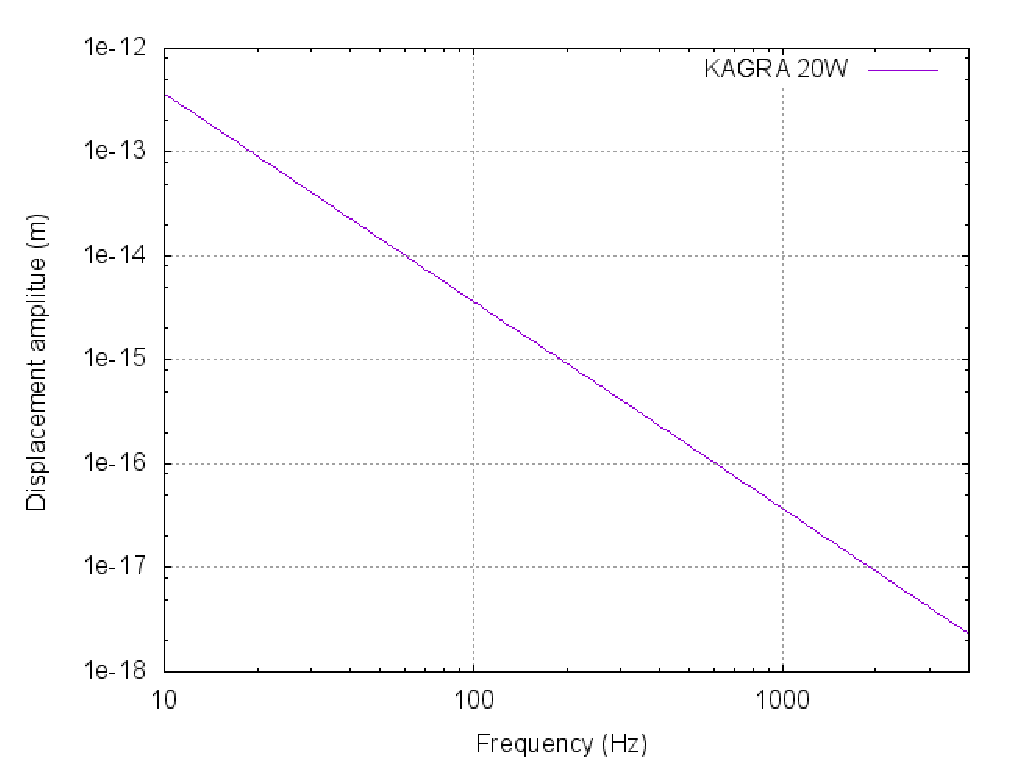
\includegraphics[width=10cm]{Figures/pcal_disp.eps}
\caption{Frequency dependence of maximum displacement by KAGRA Pcal. 
Assumption 1: Using total laser power to one frequency.
Assumption 2: pessimistic estimation of transmitter module optical efficiency and 
AOM diffraction efficiency (total 50$\%$). }
\label{fig:kagra_pcal_displacement} 
\end{center}
\end{figure}

 
%----------------------------------------------------------------------------------------

\section{Purpose of photon calibrator}
\subsection{Interferometer Calibration}

One of the main calibration method to reconstruct $\Delta L_{\rm ext}$, differenctial arm length (DARM), 
uses the combination of obtained error signal($d_{\rm err}$) and feedback signal($d_{\rm ctrl}$) 
with considering the slow temporal variations in 
aLIGO~\cite{LIGO-CAL,Tuyenbayev}.
%\footnote{The detail document is https://arxiv.org/pdf/1608.05134.pdf}. 
In this document, we assume the LIGO DARM control system which is shown in Figure~\ref{fig:L_DARM_control_loop}
({\bf Ask experts how to control in bKAGRA, especially Actuator part}). 
\begin{figure}
\begin{center}
%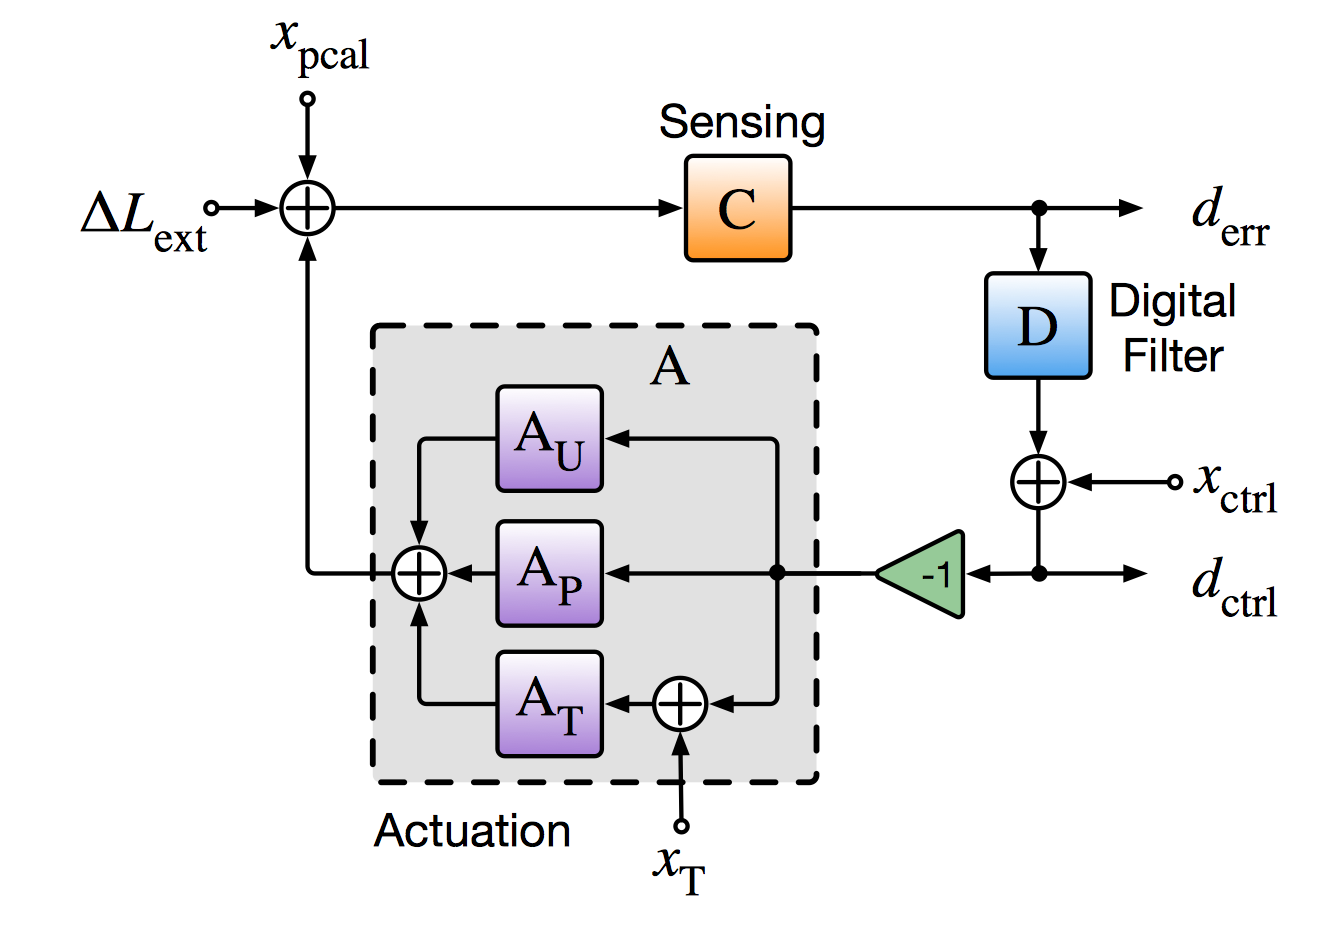
\includegraphics[width=8cm]{Figures/L_DARM_control_loop.eps}
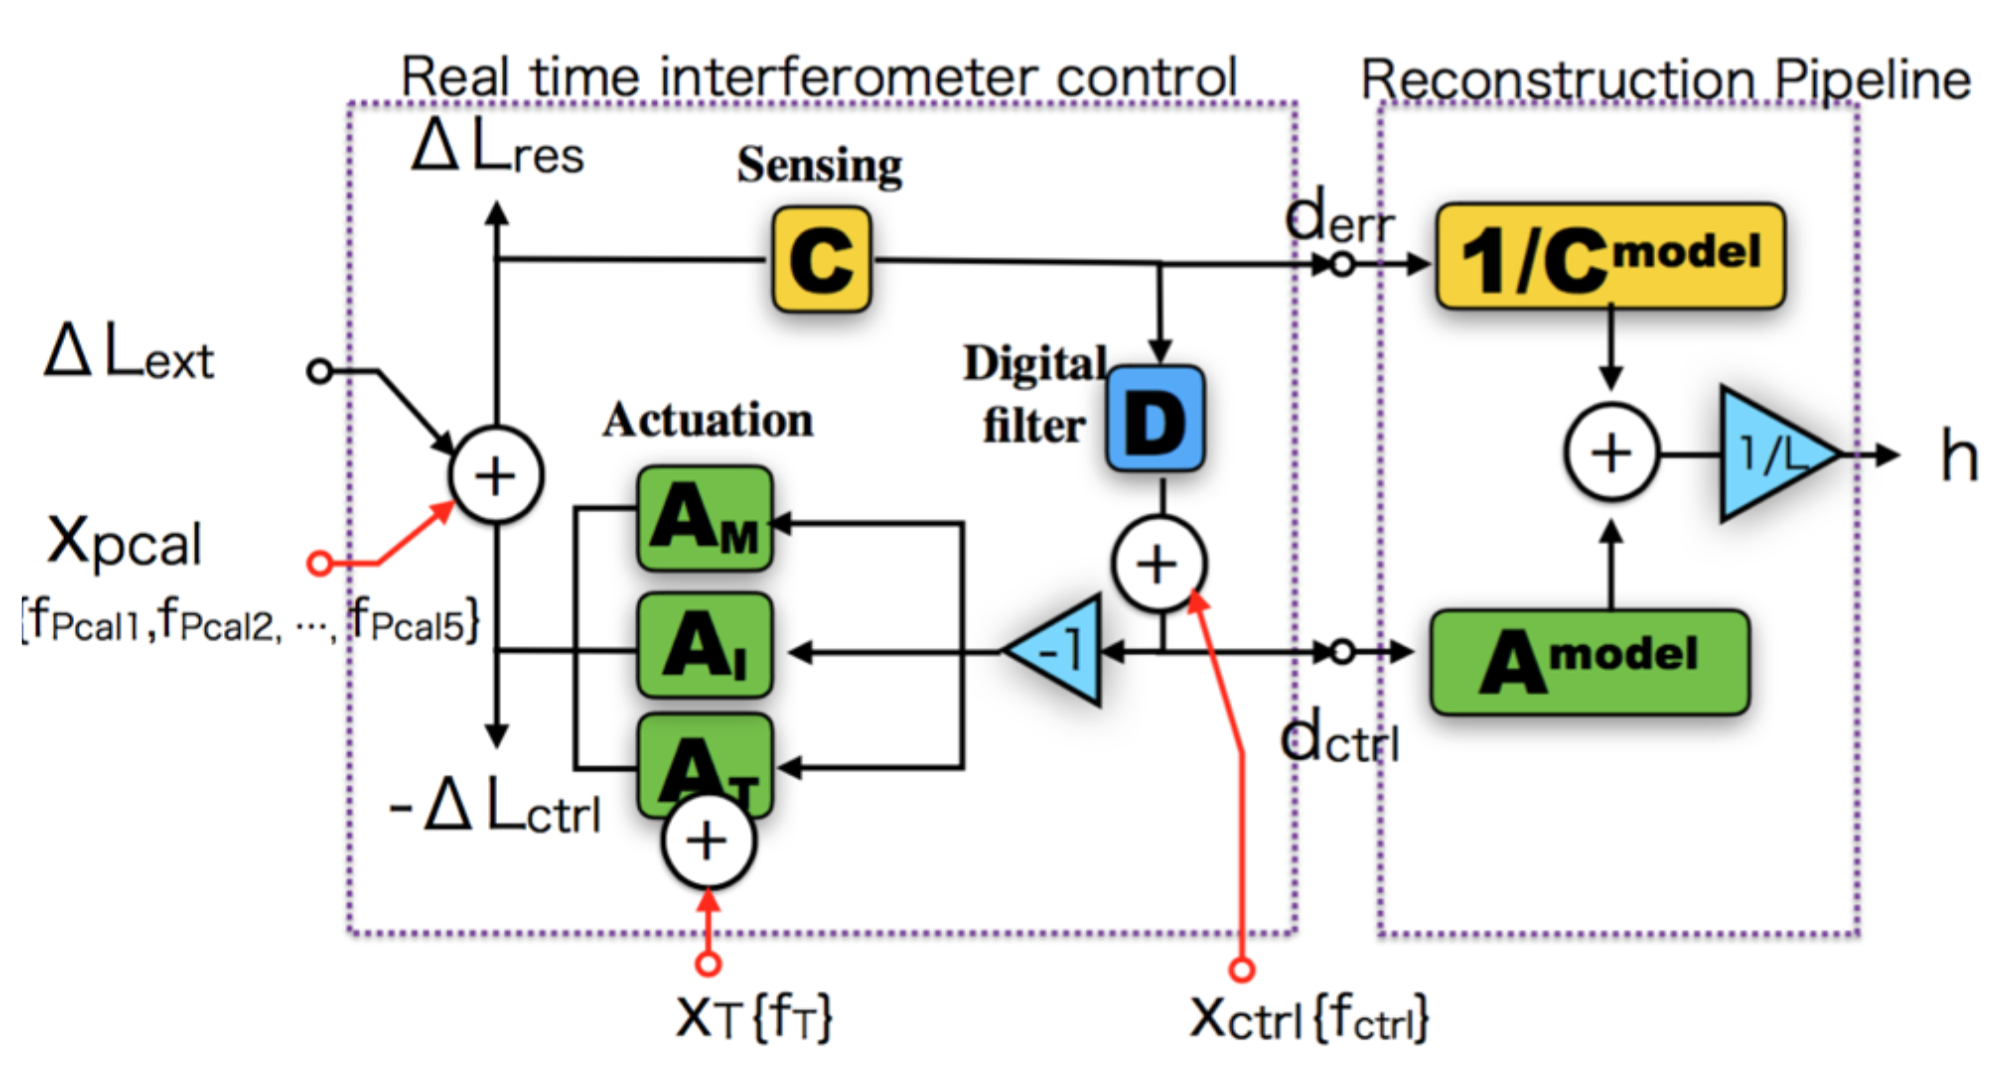
\includegraphics[width=10cm]{Figures/DARM_loop_and_CAL.eps}
%\caption{Schematic diagram of the LIGO DARM control loop.}
\caption{Schematic diagram of the real-time interferometer differential 
arm (DARM) control loop and calibration pipeline adopted 
from~\cite{LIGO-CAL,Tuyenbayev}.}
\label{fig:L_DARM_control_loop} 
\end{center}
\end{figure}
This servo is described in term of 
(i) sensing function, $C(f,t)$ 
(ii) digital filters, $D(f)$ 
(iii)actuation function, $A(f,t)$, 
and $G(f,t) = C(f,t)D(f)A(f,t)$ is the DARM open loop transfer function  

The sensing function$C(f,t)$ can be written in
\begin{equation}
C(f,t) = \frac{\kappa_{\rm C}(t)}{1+if/f_{\rm C}(t)}Q(f) \equiv P(f,t) Q(f).
\end{equation}
$Q(f)$ is the time-independent part of the sensing function, which includes
photodetector response,
electronic response
and signal delay caused by light traveling time of interferometer arm.
$P(f,t)$ is the time-dependent part of the sensing function, which includes
optical gain sale factor, $\kappa_{\rm C}(t)$ and coupled-cavity response.
Coupled-cavity response is approximated by a single pole ($f_{\rm C}(t)$).

The actuation function$A(f,t)$ can be written in
\begin{equation}
A(f,t) = \kappa_{\rm PU}(t)(A_{\rm P,0}(f)+A_{\rm U,0}(f)) + \kappa_{\rm T}(t) A_{\rm T,0}(f).
\end{equation}
$A_{\rm P,0}(f)$, $A_{\rm U,0}(f)$ and $A_{\rm T,0}(f)$ are models of the actuation function 
of the penultimate, upper-intermediate and the test mass stage 
when both $\kappa_{\rm PU}(t_0)$ and $\kappa_{\rm T}(t_0)$ are set to 1.

To monitor those four time variation parameters, 
$\kappa_{\rm C}(t)$, $f_{\rm C}(t)$, $\kappa_{\rm PU}(t)$ and $\kappa_{\rm T}(t)$, 
we need to inject modulated excitations into the DARM loop.
Also, to measure the $\kappa_{\rm C}(t)$ individually form $\kappa_{\rm PU}(t)$ and $\kappa_{\rm T}(t)$,
we need additional system to inject modulated excitations to ETM.
Photon calibrator is powerful tool for this purpose.
So, we should inject following four modulated excitations;
(i) two modulated excitations using a photon calibrator system ($x_{\rm pcal1}$ and $x_{\rm pcal2}$)
(ii) one modulated excitations into the overall DARM actuation ($x_{\rm ctrl}$)
(iii) one modulated excitations into the test mass stage actuation ($x_{\rm T}$).
The responses in $d_{\rm err}$ at time $t=t'$ for each modulated excitations can be written by
\begin{eqnarray}
d_{\rm err, t'}(f_{\rm pcal1}) &=& \frac{C(f_{\rm pcal1},t')}{1+G(f_{\rm pcal1},t')} x_{\rm pcal1} \\
d_{\rm err, t'}(f_{\rm pcal2}) &=& \frac{C(f_{\rm pcal2},t')}{1+G(f_{\rm pcal2},t')} x_{\rm pcal2} \\
d_{\rm err, t'}(f_{\rm ctrl}) &=& \frac{-A(f_{\rm ctrl}, t')C(f_{\rm ctrl},t')}{1+G(f_{\rm ctrl},t')} x_{\rm ctrl}  \\
d_{\rm err, t'}(f_{\rm T}) &=& \frac{\kappa_{\rm T}(t') A_{\rm T,0}(f_{\rm T}, t')C(f_{\rm T},t')}{1+G(f_{\rm T},t')} x_{\rm T} 
\end{eqnarray}
Using $x_{\rm pcal1}$ and $x_{\rm T}$ modulated excitations, $\kappa_{\rm T}(t')$ is obtained.
Using $x_{\rm ctrl}$ modulated excitation and $\kappa_{\rm T}(t')$, $\kappa_{\rm PU}(t')$ and $A(f,t')$ are obtained. 
Using $x_{\rm pcal2}$ modulated excitation and $A(f,t')$, $\kappa_{\rm C}(t')$ and $f_{\rm C}(t')$ are obtained.

Finally, $\Delta L_{\rm ext}(t)$ is reconstructed by following equation:
\begin{eqnarray}
\Delta L_{\rm ext}(t) = &[{\cal P}(f_{\rm C}(t))/ \kappa_{\rm C}(t) * {\cal Q} ]^{-1} * d_{\rm err}(t) \nonumber \\
& + [ 
  \kappa_{\rm PU}(t)({\cal A}_{\rm P,0} + {\cal A}_{\rm U,0}) + \kappa_{\rm T}(t) {\cal A}_{\rm T,0}  
]
* d_{\rm ctrl}(t),
\end{eqnarray}
where ${\cal P}(f_{\rm C}(t))$, ${\cal Q}$, ${\cal A_{\rm P,0}}$, ${\cal A_{\rm U,0}}$ and ${\cal A_{\rm T,0}}$  
are the time-domain filters created from $P(f,t)$, $Q(f)$, $A_{\rm P,0}(f)$, $A_{\rm U,0}(f)$ and $A_{\rm T,0}(f)$, and $*$ denotes convolution.

To reduced the systematic uncertainty, frequencies of modulated excitations are selected with following conditions:
(1) Frequencies of $x_{\rm pcal1}$ , $x_{\rm ctrl}$ and $x_{\rm T}$ should be in a narrow frequency band.
(2) Such frequency band should be selected where the magnitude of the transfer functions of 
the combined penultimate and upper intermediate mass stage and the test mass stage are 
approximately equal.
(3) Frequencies of $x_{\rm pcal2}$ should be near the coupled-cavity pole frequency.


\subsection{Hardware injection test}
Hardware injection test is one of the important end-to-end test which 
inject various waveforms to end test mass.
To analyze the hardware injection test data, we perform 
detector performance, data acquisition system, calibration system, 
data transfer system, data analysis pipeline.
We can obtain the waveforms with detector response, so 
various information will be obtained through hardware injection test.
\begin{itemize}
\item test of calibration system\\
We can test the strain signal calibration accuracy of 
sign, amplitude, phase and timing.
\item check of analysis tools\\
To inject the gravitational wave signals such as inspiral signal from 
compact binary coalescence, we can check the analysis tools/pipeline 
and systematic error due to calibration accuracy.
\item injection of complex signals\\
To inject complex signals such as supernovae waveform, Cosmic string waveform, ringdown waveform, 
we can judge that complex signals can observe correctly or not. 
If we understood that there are un-observable signal, we can consider the update of observation scenario or
calibration system.
\item blind injection\\
\end{itemize}
When we apply hardware injection test, it will be better to inject signal without DARM control loop.
The reasons are (i) limited by the fluctuation of feedback signals (ii) uncertainty of actuation efficiency
(iii) uncertainty of higher frequency injection 
(We don't know higher frequency injection by actuator works well or not.)
Photon calibrator is also powerful tool for hardware injection test.
To measure the laser power and to check the performance of AOM, we achieved the accurate hardware injection test.

\subsection{Photon pressure actuator}

%----------------------------------------------------------------------------------------

\section{Calibration line of KAGRA}
%% Equation of total laser power for calibration line
%% (depend on calibration line frequency, sensitivity, signal-to-noise ratio)


%----------------------------------------------------------------------------------------

 
% Chapter 1

\chapter{Instruments overview} % Main chapter title

\label{Chapter3} % For referencing the chapter elsewhere, use \ref{Chapter1} 



%----------------------------------------------------------------------------------------

\section{Layout of Photon calibrator}
The KAGRA photon calibrator is placed around EXA/EYA chamber, which is installed 36 m away from the end test mass (ETM). We push the mirror surface with the modulated photon pressure directly. Figure \ref{fig:Pcal_overview} shows the layout of the KAGRA photon calibrator. The photon calibrator consists of transmitter module (Tx module), receiver module (Rx module), periscope, and telephoto camera module (TCam module). We place the 20~W laser in Tx module, whose frequency is 1047 nm. The 1064 nm laser is not used due to avoid the coupling with main beams.   The power of the laser is modulated by the optical follower servo (OFS). We split the beams in Tx module for pushing the drum head node points of the ETM due to elastic deformation. We transfer the beams to the ETM though the periscope. All the periscope structures are placed into the EXA/EYA chamber. The beam is received by the Rx module. We place a 6 inches integrating sphere for the accurate measurement of the laser power and two quadrant photo detector (QPD) for the beam position monitor. We also measure the beam position on the ETM surface using the telephoto camera (TCam). The Tcam is consists of the astronomical telescope, focuser, and high resolution digital camera.  Details of instruments are described following section.
\begin{figure}
\begin{center}
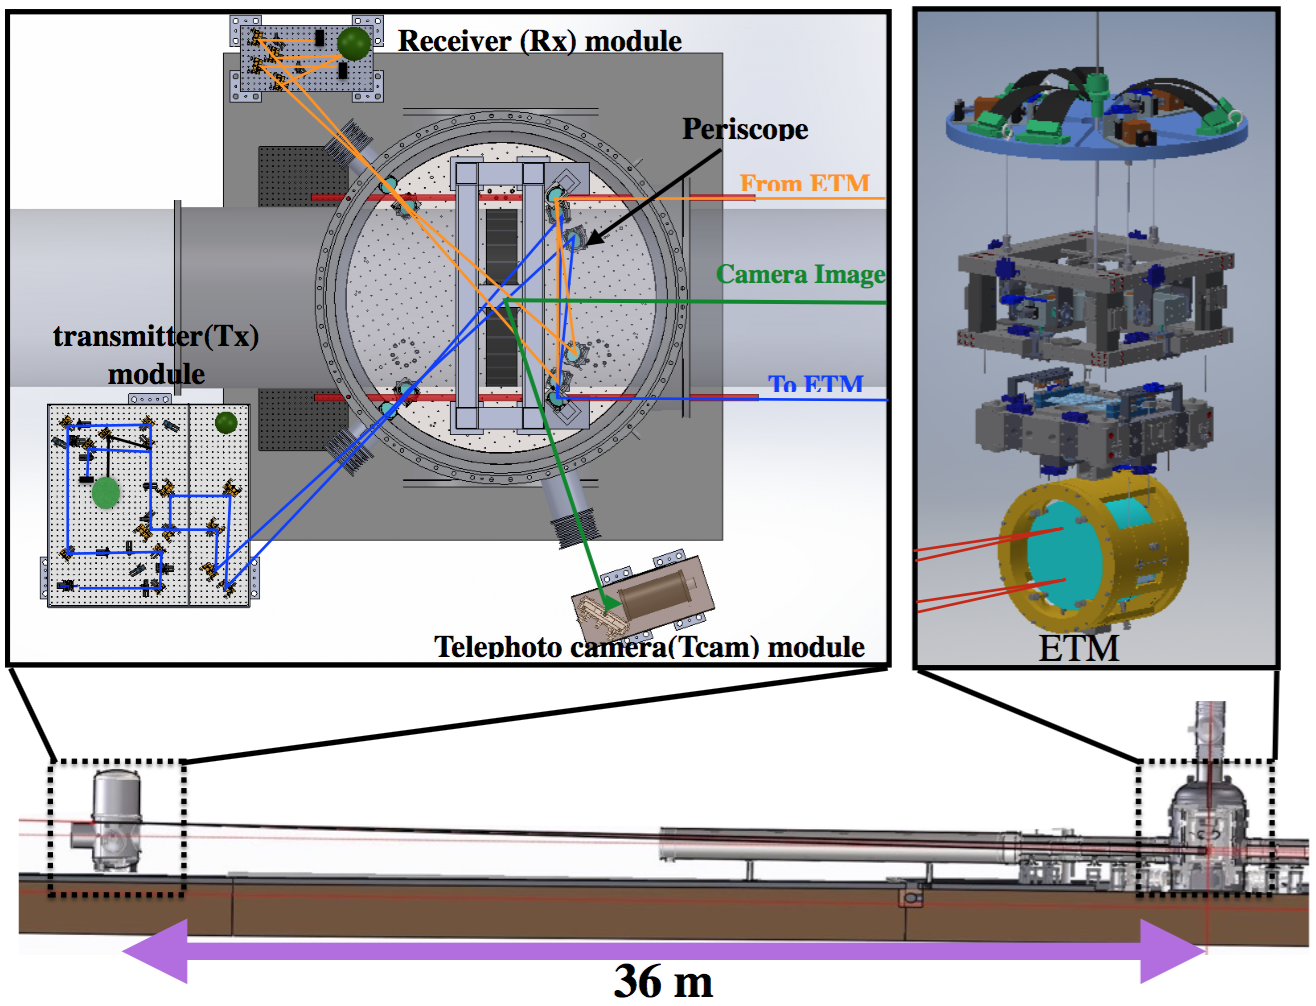
\includegraphics[width=14cm]{Figures/Pcal_overview.eps}
\caption{KAGRA photon calibrator. The calibration system is placed around the EXA/EYA chamber. We mount the optical lever and optical baffle as well.} 
\label{fig:Pcal_overview} 
\end{center}
\end{figure}

%----------------------------------------------------------------------------------------

\section{Transmitter (Tx) module}
The Tx module is placed at the side of the EXA/EYA chamber. Figure~\ref{fig:Tx_module_overview} shows the view of Transmitter module. All the optical components are mounted on the $900~\mathrm{mm}\times  900~\mathrm{mm}$ breadboard (B9090L; Thorlabs). The bread board is placed on the support structure. The electrical module for the control and readout are also hosed in the support structure. 

\begin{figure}
\begin{center}
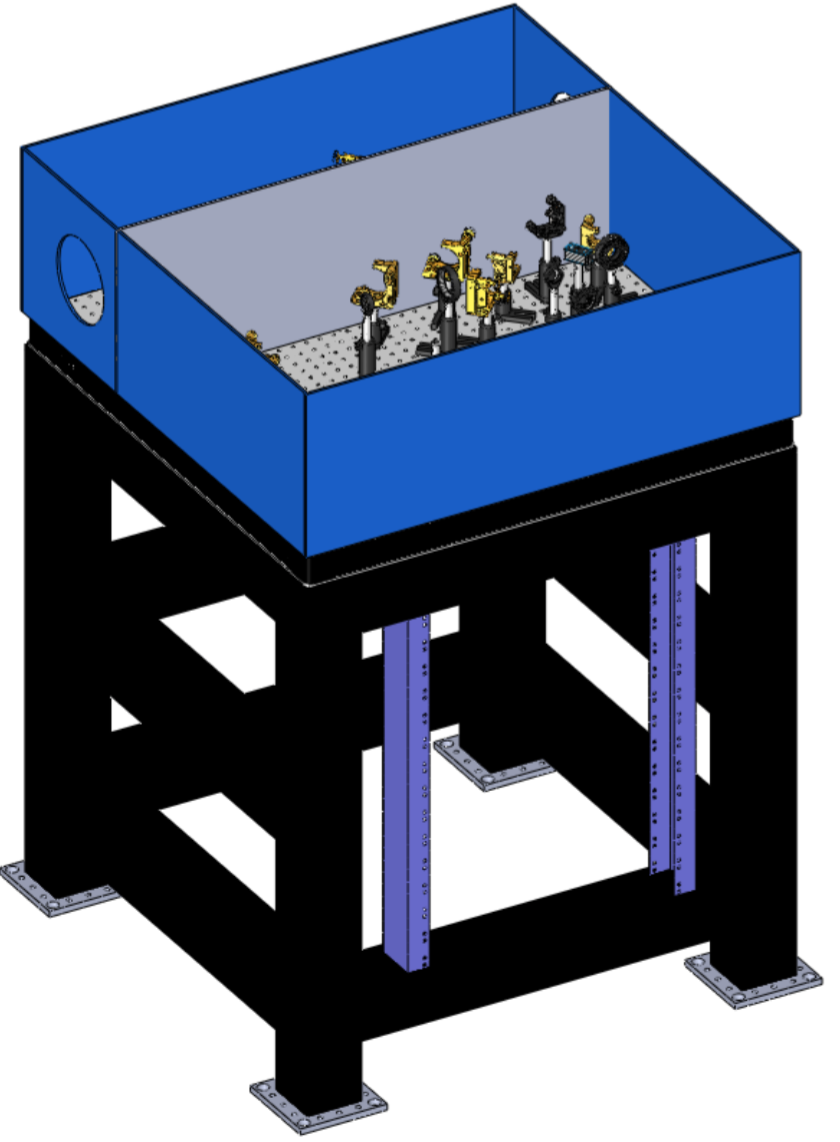
\includegraphics[width=8cm]{Figures/Tx_module_overview.eps}
\caption{.} 
\label{fig:Tx_module_overview} 
\end{center}
\end{figure}

Figure~\ref{fig:Tx_module_layout} shows the optical layout of Tx module. All the optical components are listed in Table \ref{tab:item_list}.

\begin{figure}
\begin{center}
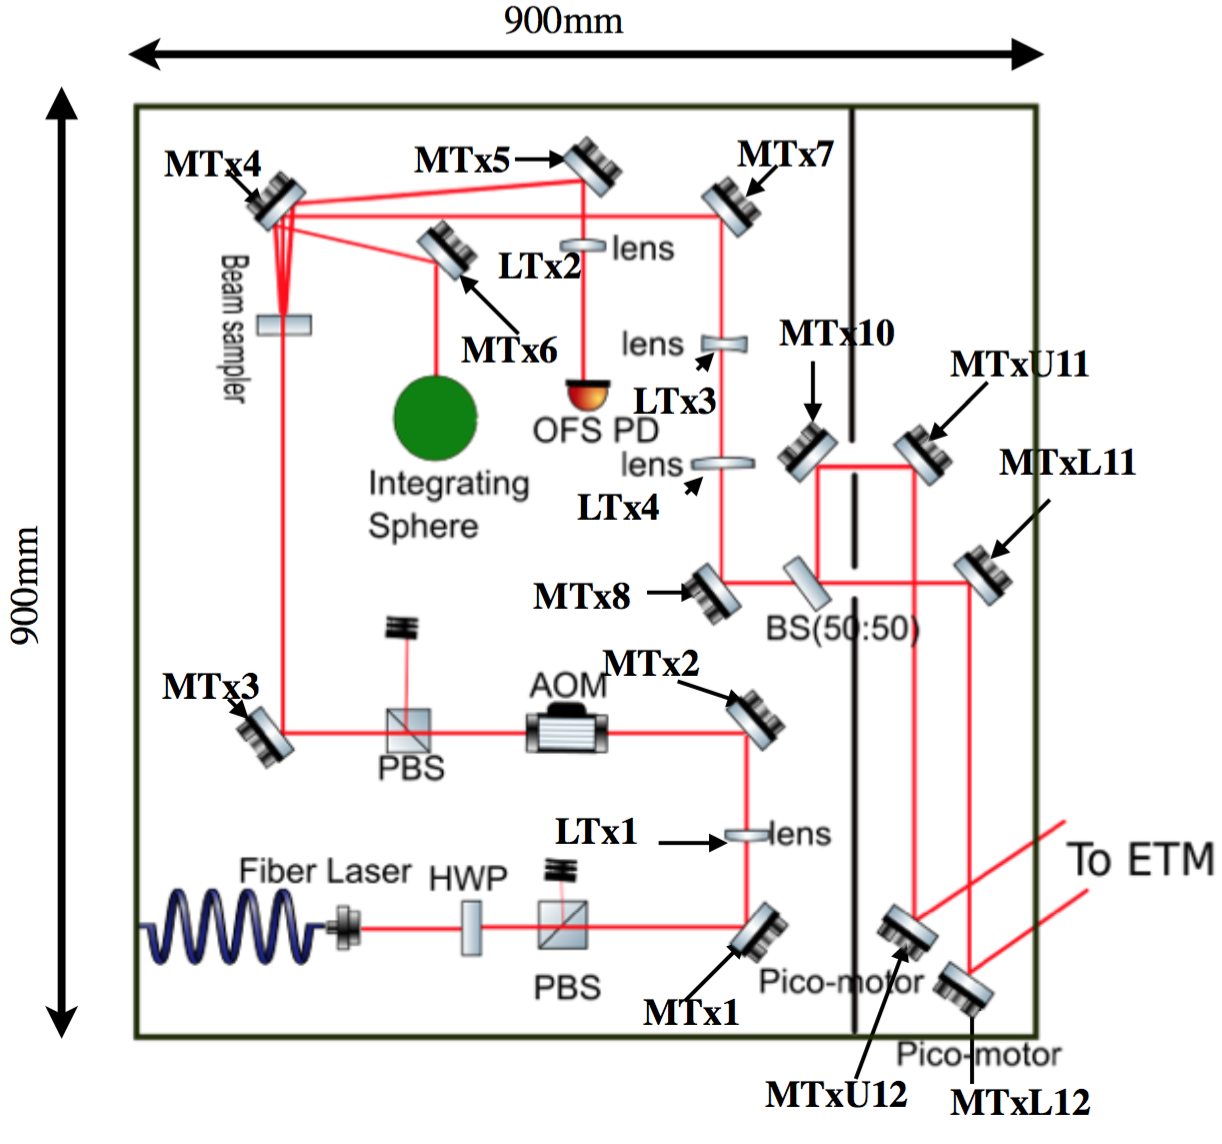
\includegraphics[width=8cm]{Figures/Tx_module_layout.eps}
\caption{.} 
\label{fig:Tx_module_layout} 
\end{center}
\end{figure}

\begin{table}
\caption{.}
\label{tab:item_list}
\centering
\begin{tabular}{ lclc|c|}
\toprule
\tabhead{\#} & \tabhead{Name} & \tabhead{Type} \\
\midrule
1 &Fiber laser & CYFL-TERA-20-LP-1047-AM1-RGO-OM1-T305-C1\\
\bottomrule\\\\
\end{tabular}
\end{table}

\subsection{Fiber laser}
We employ the CW fiber laser made by the LER photonics as shown in Fig.~\ref{fig:Laser}. The maximum power and frequency are 20 W and 1047 nm, respectively. The model number of the laser is CYFL-TERA-20-LP-1047-AM1-RGO-OM1-T305-C1. The maximum laser power of KAGRA Pcal is 10 times larger than that of LIGO. This is because that we need the high power laser for the injection test and photon pressure actuator technique. The typical beam width of the laser is 0.5~mm when we mount the isolator. We summarize the specification of the laser as shown in Table~\ref{tab:Laser_spec}.

\begin{figure}
\begin{center}
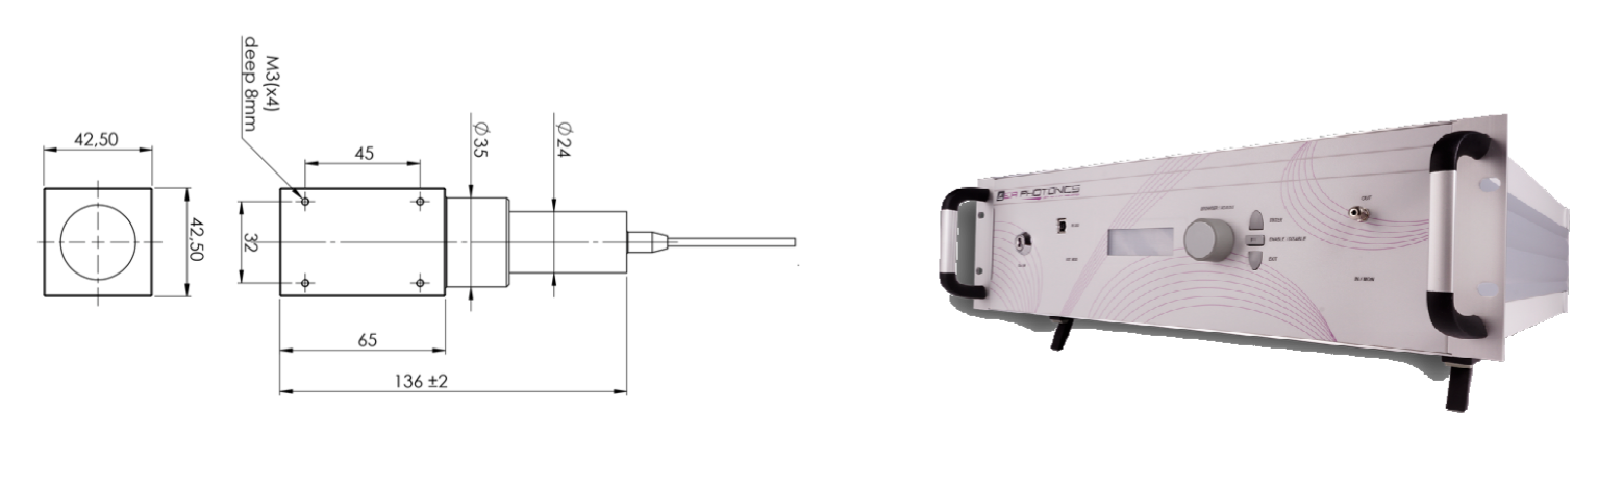
\includegraphics[width=14cm]{Figures/Laser.eps}
\caption{The fiber laser and drawing of isolator.} 
\label{fig:Laser} 
\end{center}
\end{figure}

\begin{table}
\caption{Specification summary of CW fiber Laser.}
\label{tab:Laser_spec}
\centering
\begin{tabular}{ ccccc}
\toprule
\tabhead{Charactaristic} & \tabhead{Typical value} & \tabhead{Unit} & \tabhead{Note} \\
\midrule
Operating central wavelength & 1047 & nm & $\pm1~\mathrm{nm}$\\
CW output power & 20 & W & \\
Output signal line-width & 0.5 & nm & FWHM\\
Output power stability & $\pm1$&\%RMS& Output power: 20~W\\
Output power tunability & 10-100&\%& \\
Optical polarization & Linier&& \\
Polarization extinction ratio & 15&dB& \\
Output fiber & PLMAFUD3460&& Nufurn company \\ 
Output fiber length & 2&m&  \\
Beam diameter & 0.5&mm& with isolator  \\
Beam quality & 1.1&$M^2$&   \\
Control & Active current control,&&   \\
mode & Active power control&&   \\
Beam quality & 1.1&$M^2$&     \\
Supply voltage & 84-264&V&AC 47 to 63 Hz   \\
Power consumption & 650&W&   \\
Housing & 448x451x132.5&mm&   \\
Total weight & 13&kg&   \\
Cooling & Air cooled with fans&&   \\
Operating temperature & 15-35&&   \\
Humidity & 5-85&\%&   \\
\bottomrule\\
\end{tabular}
\end{table}

\subsection{Beam shutter}
We have to pay attention to safety for the operation of the high power laser. In order to dump the beam, we use the beam shutter made by lasermet company. The model number of the shutter is LS-10-12. The aperture size and  Max laser power are 15 mm and 20 W. These number meet our requirement due to the laser spot size and maximum power. We control the beam shutter on the GUI. The specification of the beam shutter is shown in Table.~\ref{tab:Beam_shutter_spec}.

\begin{table}
\caption{Specification of beam shutter.}
\label{tab:Beam_shutter_spec}
\centering
\begin{tabular}{ ccccc}
\toprule
\tabhead{Charactaristic} & \tabhead{Typical value} & \tabhead{Unit} & \tabhead{Note} \\
\midrule
Max laser power & 20 & W & \\
Aperture size & 15 & mm & \\
Drive voltage & 11-14 & V DC & \\
Current consumption & 150 & mA & \\
Size & $98 \times 63.5 \times 36$ & mm & \\
\bottomrule\\
\end{tabular}
\end{table}

\subsection{Half wave plate}
To control the polarization angle of incident beam, we employ the zero order half wave plate (HWP) made by the CVI laser optics. The model number of the HWP is QWPO-1047-05-2-R10 whose diameter are 12.7mm. The HWP is mounted on the rotation mount made by Thorlabs. The thick ness are optimized at 1047 nm.
The specification of the HWP is listed in Table~\ref{tab:HWP_spec}.
\begin{table}
\caption{Specification of HWP.}
\label{tab:HWP_spec}
\centering
\begin{tabular}{ ccccc}
\toprule
\tabhead{Charactaristic} & \tabhead{Typical value} & \tabhead{Unit} & \tabhead{Note} \\
\midrule
Waveplate Type & Quartz Waveplates &  & \\
Wavelength Range & 1047 & nm & \\
Retardance & $\lambda/2$&  & \\
Clear Aperture & 85 & \% & of diameter \\
Reflection & 0.25 & \% & \\
Retardance Tolerance & λ/200 to λ/500 & & at 23Degree C \\
Material & Crystal Quartz &  & \\
Surface Quality & 10-5  & scratch-dig & \\
Waveplate Diameter & 12.7 & mm & \\
\bottomrule\\
\end{tabular}
\end{table}

\subsection{Polarizer}
We place two polarizers to define the polarization angle accurately. This is because that the power of the laser is modulated by acousto-optic modulator (AOM) whose performance strongly depend on the incident polarization angle.
One polarizer is placed behind HWP. Another one is placed after AOM. The Polarizer is made by Karl-Lambrecht. We purchased TFPC12-1047 that is optimized at 1047 nm. 
\subsection{Lens}
We have dane a mode matching simulation using JamMt. We assumed laser beam to be gaussian distribution. We have to place the focus of the laser at the AOM. Thus, we decide the optimal position and focal length of the 1 inch lens (L1), where the assumed beam waist of the fiber laser and AOM are 0.5 mm and XXX mm, respectively. 
Furthermore, we place two lenses for placing the focus at the surface of the ETM. We employ the combination of 1 inch negative lens and 2 inch positive lens. The Gaussian beam can describe the following relation:
\begin{equation}
w(z)=\omega_0\sqrt{1+\left( \frac{\lambda z}{\pi \omega_0^2}\right)^2},
\end{equation}
where $\lambda$ is wavelength of the laser, $w_0$ is beam waist, $z$ is direction from the focus. We estimate the minimum differential beam spot by changing beam waist because it make the alignment easier. The minimum beam spot is written by 
\begin{equation}
\left .\frac{dw(z)}{dw_0} \right|_{z=36m}=0.
\end{equation}
The estimated beam waist and beam spot is 3.5 mm and 5.5 mm as shown in Fig. XXXX.
We also place the lens at the front of the photo detector for the OFS. The parameters of the simulation results are listed in Table.~\ref{tab:Tx_lenses_spec}. All lenses are made by CVI laser optics. The material of lenses are fused silica. The AR coating is placed at both surface. 

\begin{table}
\caption{Specification of lenses.}
\label{tab:Tx_lenses_spec}
\centering
\begin{tabular}{ ccccc}
\toprule
\tabhead{Lens number} & \tabhead{part number}& \tabhead{Diameter [mm]} & \tabhead{Focal length}  \\
\midrule
L1 &  & 25.4 & \\
L2 &  & 25.4& \\
L3 &  & 25.4 & \\
L4 &  & 50.8 & \\
\bottomrule\\
\end{tabular}
\end{table}

\subsection{Mirror}
We employ nine 1 inch mirrors and four 2 inch mirrors. The 1 inch mirror is made by CVI laser optics. They place the HR coating on the surface of mirror. On the other hand, we use the HR coating on the fused silica disc of 2 inch in diameter. The coating and polishing the fused silica is made by Sigma-koki corporation. The reflectance of the mirror is shown in Figure. XXXX.
 The reflectance of HR coating depends on the incident angle and the polarization angle. We labeled mirrors as M-Tx1 toM-Tx-11, M-Tx-t-1,M-Tx-t-2, and M-Tx-b-1. The specification of mirrors are summarized in Table.~\ref{yab:Tx_mirror_spec}. All mirror is aligned with optical mirror mount made by Newport company.
 
 \begin{table}
\caption{Specification of Mirrors.}
\label{tab:Tx_mirror_spec}
\centering
\begin{tabular}{ ccccc}
\toprule
\tabhead{Mirror number} & \tabhead{part number}& \tabhead{Diameter [mm]} & \tabhead{Polarization}  \\
\midrule
M-Tx-1 &  &25.4  & \\
M-Tx-2 &  &25.4  & \\
M-Tx-3 &  &25.4   & \\
M-Tx-4 &  &25.4   & \\
M-Tx-5 &  & 25.4  & \\
M-Tx-6 &  &25.4  & \\
M-Tx-7 &  &25.4   & \\
M-Tx-8 &  &25.4   & \\
M-Tx-9 &  &25.4   & \\
M-Tx-10 &  & 50.8& \\
M-Tx-11 &  &  50.8& \\
M-Tx-t-1 &  &  50.8& \\
M-Tx-t-2 &  & 50.8 & \\
M-Tx-b-1 &  & 50.8 & \\
\bottomrule\\
\end{tabular}
\end{table}
 
\subsection{Beam splitter}
To reduce the elastic deformation, we separate the beam with the beam splitter made by CVI laser optics for pushing the node points of mirror. The part number of beam splitter is BS1-1064-50-2025-45P. The diameter of the beam splitter is 2 inch. Table~\ref{tab:BS_spec} shows the separation ratio of beam splitter.
\begin{table}
\caption{Specification of beam splitter.}
\label{tab:BS_spec}
\centering
\begin{tabular}{ ccccc}
\toprule
\tabhead{Charactaristic} & \tabhead{Typical value} & \tabhead{Unit} & \tabhead{Note} \\
\midrule

Beamsplitter Type&Laser Line Plate Beamsplitters&&\\
Beamsplitter Shape& Round&&\\
Wavelength Range &800 &nm&\\
Bevel/Chamfer & 0.35 mm $\times$ 45 Degree &&\\
Wedge Angle Tolerance & 5& arcmin &\\
Coating Material & Laser Line Dielectric&&\\
Angle of Incidence & 45& Degree&\\
Clear Aperture & 85&\%& \\
Substrate/Material & Fused Silica&&\\
Surface Flatness & λ/10 &&\\
Surface Quality & 10-5& scratch-dig& \\
Beamsplitter Diameter & 50.8& mm&\\
Beamsplitter Thickness & 6.35 mm&&\\
Thickness Tolerance &$ \pm0.25~\mathrm{mm}$&&\\
\bottomrule\\
\end{tabular}
\end{table}

\subsection{Optical follower servo}
\subsection{Photo detector}
To detect the laser power, we use the photo detector. We place the photodetector at the working standard, Optical follower sarvo, Integrating sphere in Tx and Rx module.
We developed the photo detector as shown in Fig.xxx. We employ the InGaAs photo diode for absolute power measurement. The InGaAs diode is placed on the circuit board. The beam is collimated for the power detection reasonably. We housed the circuit board into the aluminum case coated by the alumite. 

\subsubsection{Cover}
The design of the cover is 
\subsubsection{InGaAs detector}
\subsubsection{Electrical Circuit}
We newly improved the electrical circuit of the photon detector as shown in Fig, \ref{fig:Photo_detector}. The electrical circuit is housed in the aluminum cover. We place the photo detector at the the behind of the electrical circuit. The layers of the circuit consists of 4 layer. We change the differential gain by changing the register and capacitor of the circuit. The electrical circuit are shown in Fig. XXX.
\begin{figure}
\begin{center}
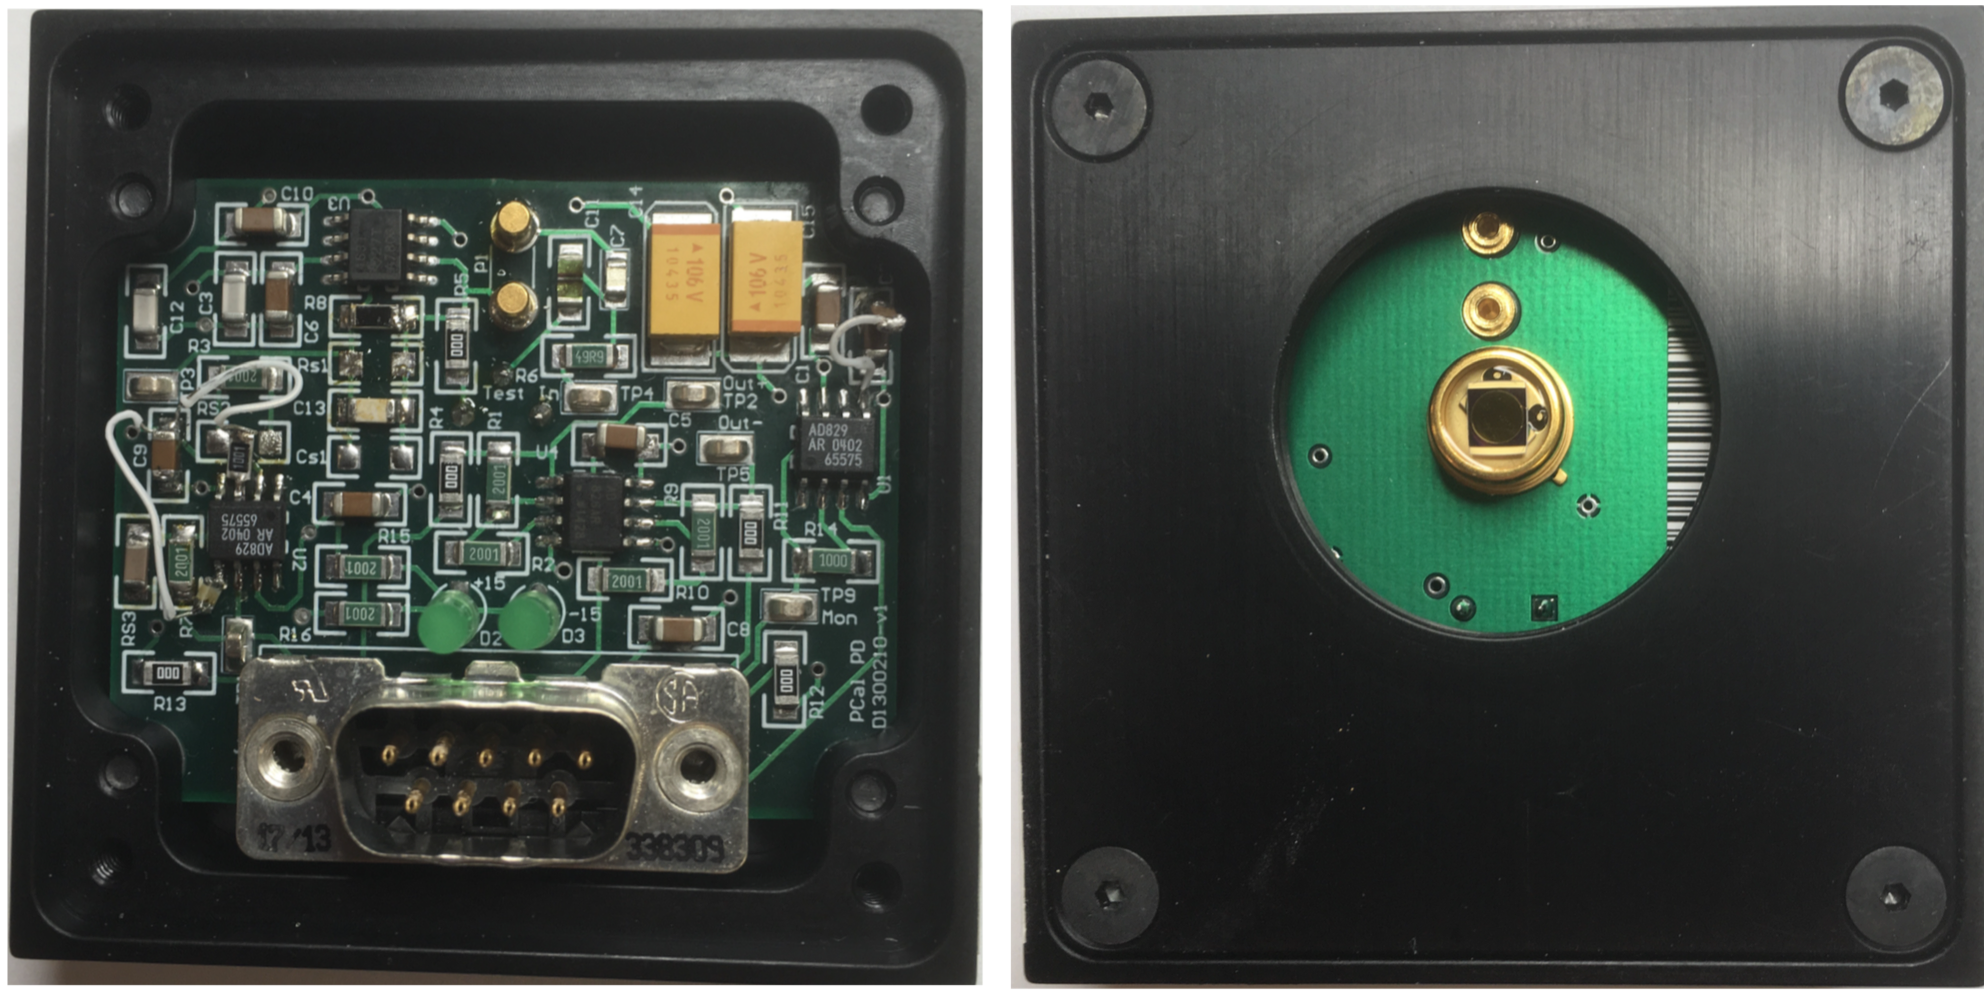
\includegraphics[width=8cm]{Figures/Photo_detector.eps}
\caption{.} 
\label{fig:Photo_detector} 
\end{center}
\end{figure}

\subsection{beam sampler}
\subsection{2 inch integrating sphere}
The 2 inches integrating sphere is used for absolute power measurement of the laser. We receive the separated laser beam at beam sampler. The typical power of the laser is XXX W. We mount the photo detector at the port of integrating sphere. The integrating sphere is made by the Lab sphere. The inner surface of the integrating sphere in mounted on the Spectralon.

\subsection{Structure}
The breadboard is placed on the support structure. The material of this structure is SUS 306. This structure can be housed electrical devices, such as driver of the fiber laser, electronics of optical follower servo, and driver of laser shutter. We simulated the resonance frequency using ANSYS. The estimated frequency is XXX Hz.

%----------------------------------------------------------------------------------------
\section{Periscope}
\subsection{Geometric optics}
\subsection{View window}
One of the serious systematic errors are optical efficiency of the view port. Therefore, we have to reduce the reflectance of  view port at least 0.1 \%. We employ the fused silica optical window whose diameter and thickness are 100 mm and 0.5 inch. We place the AR coating on both surfaces of the window. Figure~\ref{fig:Pcal_window} shows the simulated transmittance of the view port. The effective diameter of the view port is about 3 inch. The incident angle of the beams are XXXX degree. 

\begin{figure}
\begin{center}
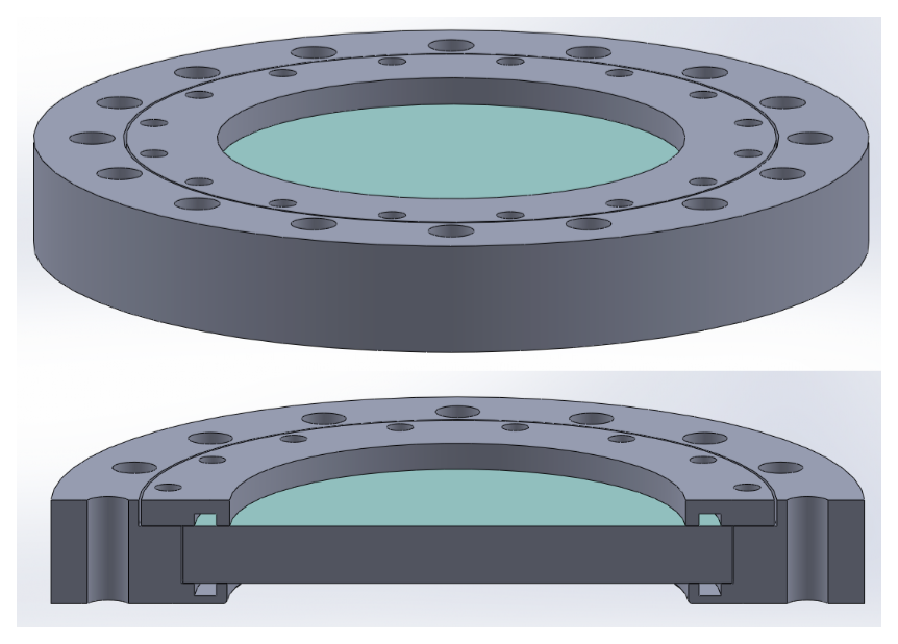
\includegraphics[width=8cm]{Figures/Pcal_view_window.eps}
\caption{.} 
\label{fig:Pcal_window} 
\end{center}
\end{figure}

The flange type of the view port is ICF152. We remodeled the blank flange of ICF 152 made by Cosmotech. Figure XXX shows the drawing of the view port. We employ the G-85 o-ring for vacuum sealing. 
\subsection{Mirrors}
We employ eight 3 inch mirrors. We place the HR coating on the polished fused silica disc. The coating and polishing the fused silica is made by Sigma-koki corporation. The reflectance of the mirror is shown in Figure. XXXX.
 The reflectance of HR coating depends on the incident angle and the polarization angle. We labeled mirrors as M1, XXXX. The specification of mirrors are summarized in Table.~\ref{tab:Periscope_mirror_spec}. All mirror is aligned with optical mirror mount made by XXXXXX.
 \begin{table}
\caption{Specification of Mirrors in periscope.}
\label{tab:Periscope_mirror_spec}
\centering
\begin{tabular}{ ccccc}
\toprule
\tabhead{Mirror number} & \tabhead{part number}& \tabhead{Diameter [mm]} & \tabhead{Polarization}  \\
\midrule
M-P-1 &  &76.2  & \\
M-P-2 &  &76.2  & \\
M-P-t-3 &  &76.2   & \\
M-P-t-4 &  &76.2   & \\
M-P-b-3 &  & 76.2  & \\
M-P-b-4 &  &76.2  & \\
M-P-5 &  &76.2  & \\
M-P-6 &  &76.2   & \\

\bottomrule\\
\end{tabular}
\end{table}
\subsection{Structure}
\subsection{Alignment}

%----------------------------------------------------------------------------------------
\section{Receiver module}
\subsection{6inch Integrating sphere}
The 6 inches integrating sphere is used for absolute power measurement of the laser. We receive the laser beam from two paths. To receive the power perfectly, we need a sufficiently large diameter hole of integrating sphere. We use for the 2 inch hole integrating sphere. We mounted the photo detector at the top of port. Details of the photo detector is explained in XXXXX.

\subsection{Mirror}
We employ four 2 inch mirrors. We place the HR coating made by Siguma-koki as shown in Fig. XXXX. For two mirrors, we make the AR coating on the back surface to pick up the beams. The specification of the mirrors are listed in Table~\ref{tab:Rx_mirror_spec}.
 \begin{table}
\caption{Specification of Mirrors in Rx module.}
\label{tab:Rx_mirror_spec}
\centering
\begin{tabular}{ ccccc}
\toprule
\tabhead{Mirror number} & \tabhead{part number}& \tabhead{Diameter [mm]} & \tabhead{Polarization}  \\
\midrule
M-Rx-1 &  &  & \\
M-Rx-2 &  &  & \\
M-Rx-3 &  &   & \\
M-Rx-4 &  &   & \\
\bottomrule\\
\end{tabular}
\end{table}
\subsection{Structure}
\subsection{Alignment}


\subsection{QPD}
\subsection{Structure}
The breadboard is placed on the support structure. The material of this structure is SUS 306. We simulated the resonance frequency using ANSYS. The estimated frequency is XXX Hz.

%----------------------------------------------------------------------------------------

\section{Camera module}
The beam position of the ETM surface corresponds to systematic error of the rotation and elastic deformation. To measure the beam position, we measure the mirror surface directly. However, the KAGRA EXA/EYA chambers are placed at 36m far from the ETM. Thus, we employ the combination of telescope and high resolution camera, we call telephoto camera (TCam). We are tuning with focus point of the mirror using focuser.  We place the view port and mirror between the ETM and TCam. Figure XXX shows the drawing of TCam unit.
\subsection{Camera}
Purpose of using the high resolution camera, we have to measure the beam position within 1 mm accuracy. Ww solved this problem by D810 digital camera made by Nikon. The D810 reprises the 36-megapixel resolution with $35.9 \times 24.0~\mathrm{mm}$ CMOS sensor. We remove the IR filter because the commercial camera is not sensitive to laser wavelength (1047 nm).
\subsection{Telescope}
We employ the Maksutov-Cassegrain type telescope for observing the ETM surface. The diameter of the primary mirror is 127 mm and its focal length is 1500 mm ($f/12$). The telescope is manufactured by Sky-watcher company. The diameter of the telescope is limited by the that of the view window size. 
\subsection{Focuser}
A focuser, which is made by Moonlight, is used for the automatic focus control. 
We connect focuser between telescope and camera. The model number is XXXXX.
\subsection{View window}
The flange type of the view port is ICF203. We remodeled the blank flange of ICF 203 made by Cosmotech. Figure~\ref{fig:Camera_window} shows the drawing of the view port. We employ the G-135 o-ring for vacuum sealing. 

\begin{figure}
\begin{center}
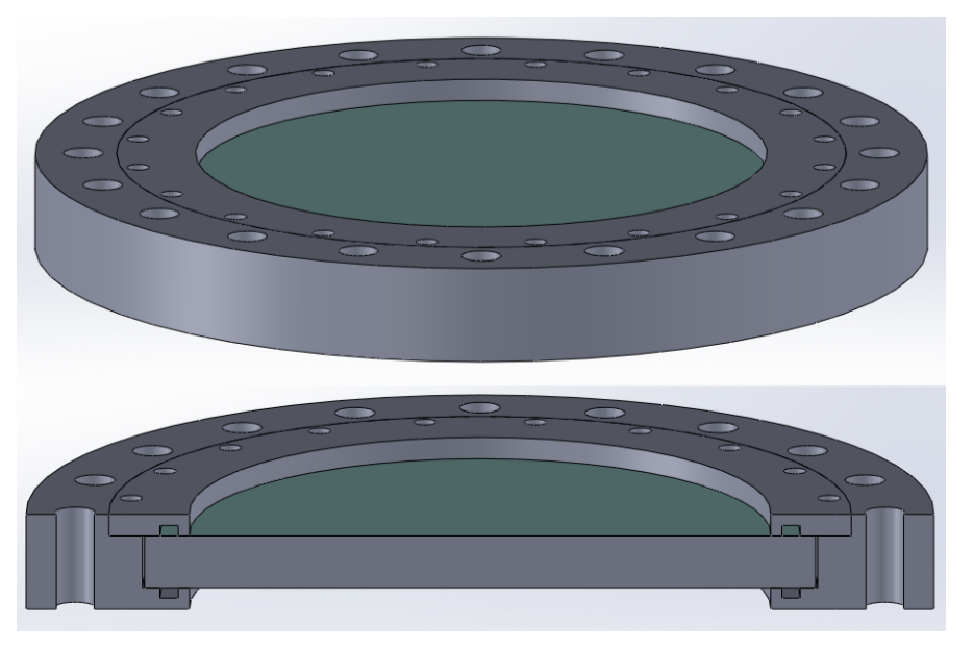
\includegraphics[width=8cm]{Figures/Camera_view_window.eps}
\caption{.} 
\label{fig:Camera_window} 
\end{center}
\end{figure}
\subsection{Mirror}
We place the mirror in the EXA/EYA chamber. The mirror size is $100 \times 80 mm$, which is mounted on the aluminum holder and optical mount. The mirror is made by Thorlab.The reflectance of the mirror is shown in Fig XXXX.
\subsection{Illuminator}
%----------------------------------------------------------------------------------------

\section{Summary}

% Chapter 1

\chapter{Elastic deformation} % Main chapter title

\label{Chapter4} % For referencing the chapter elsewhere, use \ref{Chapter1} 
%The elastic deformation is one of the serious systematic error in Photon calibrator.
Calibration of interferometer above 1kHz is a challenging task. 
It was demonstrated that the calibration forces applied by a centered 
photon calibrator beam produce local elastic deformations which 
significantly alter the sensed displacement of the 
interferometer~\cite{Hild:2007,Goetz:2009}.
Even stiff materials like fused silica or sapphire experience small 
deformation when photon calibrator forces are applied. The response to 
the excitation forces can be represented by the appropriate linear 
combination of normal modes. These effects, however, can be mitigated 
by applying at least two beams diametrically opposed and sufficiently 
displaced from the center of the test mass. 
This scheme was tested and implemented in LIGO and advanced LIGO photon 
calibrator~\cite{Daveloza,Karki}.
In this chapter, the investigations to identify 
the modes and their effect on the calibrator performance are discussed.  

%\section{Free mass motion}
%\section{Transfer function}
%\section{Modal analysis}

\section{Finite Element Analysis}
The modal analysis and simulation of the elastic deformation are made 
by using Finite Element Analysis (FEA) software package, ANSYS~{ANSYS}.
Figure~\ref{fig:elmodes} shows the summary of primary modes, drumhead and 
butterfly modes compared between KAGRA and LIGO.
Figure~\ref{fig:edeform} shows the displacement between the sensed motion 
and rigid-body motion as a fundtion of frequency for optimally positiond 
beams on KAGRA test mass, as well as $\pm$1 mm and $\pm$3 mm offsets from 
the optimal positions.

\begin{figure}
\begin{center}
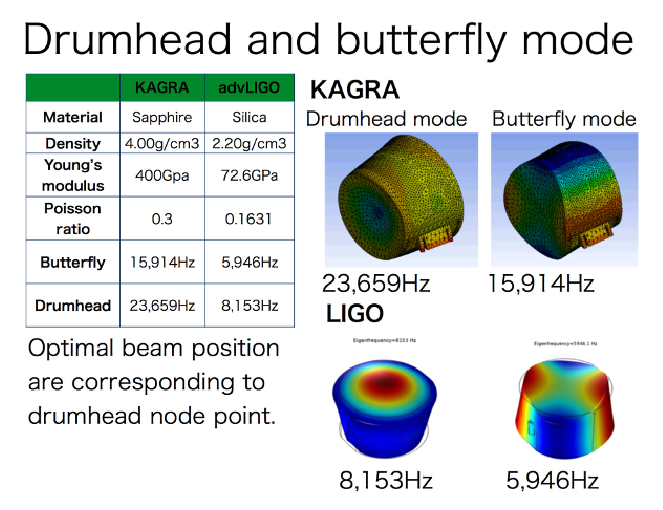
\includegraphics[width=14cm]{Figures/elmodes.eps}
\caption{Summary of drumhead and butterfly modes on KAGRA test mass 
compared with LIGO test mass.} 
\label{fig:elmodes} 
\end{center}
\end{figure}

\begin{figure}
\begin{center}
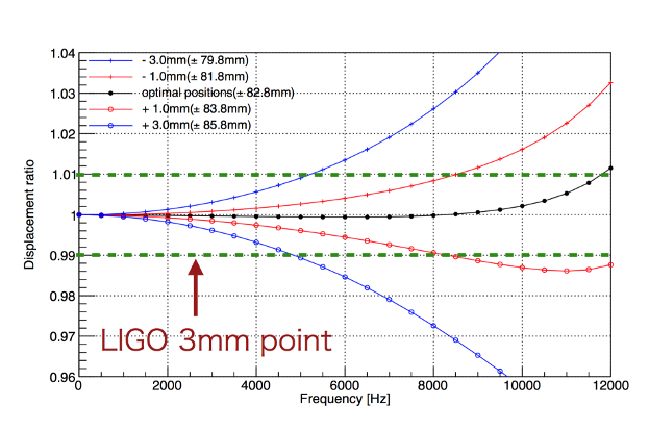
\includegraphics[width=14cm]{Figures/edeform.eps}
\caption{The ratio between the total sensed motion and rigid body motion 
as a function of frequency for optimally positoned baams and 
$\pm$1 mm and $\pm$3 mm offsets.} 
\label{fig:edeform} 
\end{center}
\end{figure}

%\section{Elastic deformation}
%\section{Summary}
 
%% Chapter 1

\chapter{Absolute power calibration} % Main chapter title
\label{Chapter5} % For referencing the chapter elsewhere, use \ref{Chapter1} 
This chapter describe the absolute power calibration procedure of KAGRA photon calibrator.
The systematic error of the absolute power is most largest in LIGO.
They measure the laser power with integrating sphere and InGaAs photodetector because displacement of mirror corresponds to laser power. 
The absolute power injected to the ETM can be obtained as average of input power at Tx module and the output power at Rx module as follows:
\begin{equation}
P=\frac{P_{TxPD}+P_{RxPD}}{2}=\frac{1+e}{2e}P_{RxPD},
\end{equation}
where $P_{TxPD}$ and $P_{RxPD}$ are the measured power of the transmitter module photo detector(TxPD) and the receiver module photodetector (RxPD), and $e=P_{TxPD}/P_{RxPD}$ is optical efficiency.
Therefore, $P_{TxPD}$ and $P_{RxPD}$ limit the calibration accuracy of the absolute displacement of the mirror.
To calibrate $P_{TxPD}$ and $P_{RxPD}$, we employ the working standard (WS) and the gold standard (GS). 

The WS of KAGRA (WSK) is the combination of integrating sphere and InGaAs photo detector (see Fig.~\ref{fig:KWS}), which is calibrated against GS of LIGO (GSL) in LHO lab as calibrated by NIST. LIGO also make working standards for LHO and LLO as shown in Fig~\ref{fig:GS_WS}.
The ratio of measured voltage of WS and GS detectors are obtained as
\begin{equation}
\frac{V_{WSK}}{V_{GSL}}.
\end{equation}
We can calibrate the response of WS using GS through this equation.

We will also use the WSK to calibrate the TxPD and RxPD, which are inside the Tx module and Rx module of Pcal, respectively. We will measure the ratio of voltage of TxPD and RxPD as follows
\begin{equation}
\frac{V_{TxPD}}{V_{KWS}}.
\end{equation}

Finally,  we obtain the calibration power $P_{GW}$ using the power standard laser in NIST.
Then, we can get the calibrated $P_{TxPD}$ and $P_{RxPD}$ as follows:

\begin{eqnarray}
P_{TxPD}=\frac{V_{TxPD}}{V_{KWS}}\frac{V_{WSK}}{V_{GSL}}P_{GS}, \\
P_{RxPD}=\frac{V_{RxPD}}{V_{KWS}}\frac{V_{WSK}}{V_{GSL}}P_{GS}
\end{eqnarray}

\begin{figure}
\begin{center}
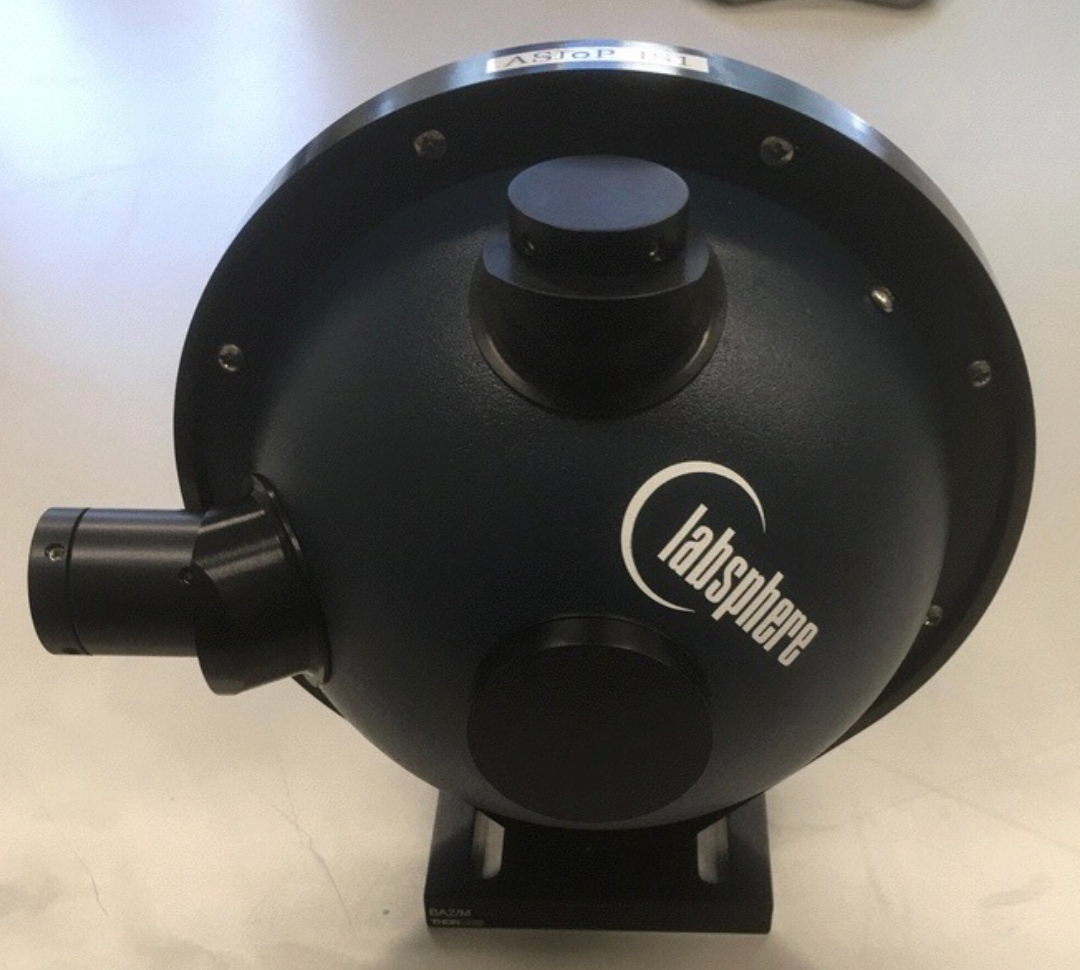
\includegraphics[width=14cm]{Figures/KWS.eps}
\caption{KAGRA working standard.} 
\label{fig:KWS} 
\end{center}
\end{figure}

\begin{figure}
\begin{center}
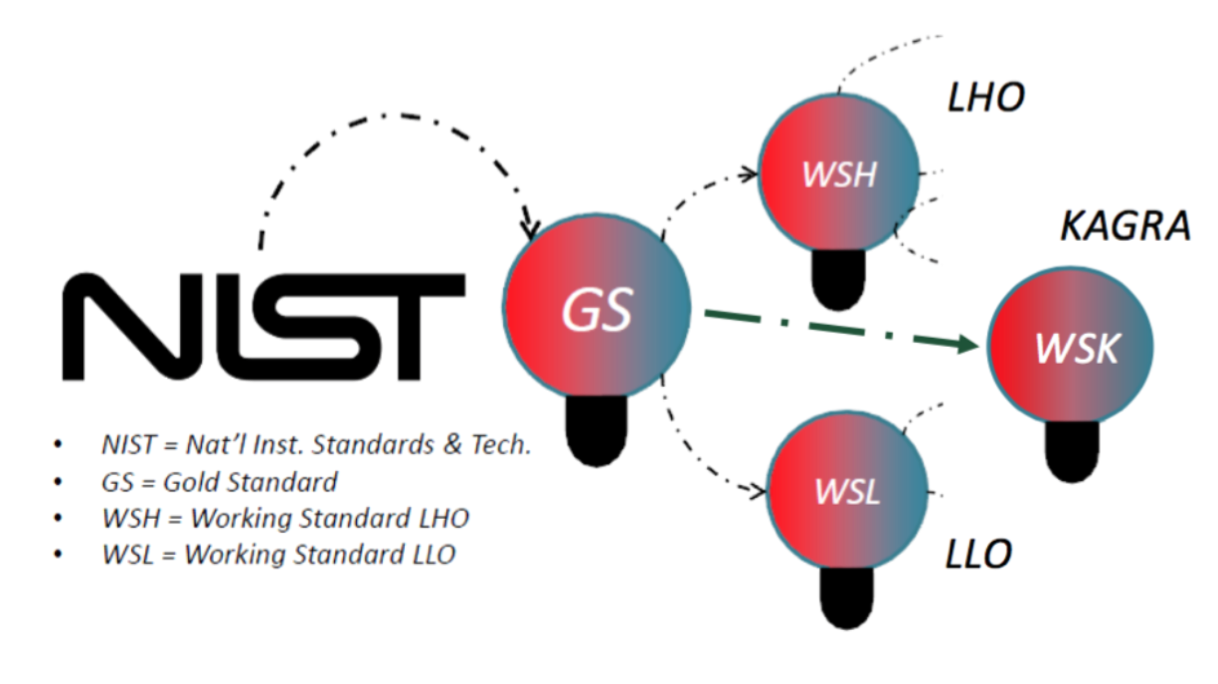
\includegraphics[width=14cm]{Figures/GS_WS.eps}
\caption{comparison with GS and WS.} 
\label{fig:GS_WS} 
\end{center}
\end{figure}

\section{Calibration in LHO}
%\begin{figure}
%\begin{center}
%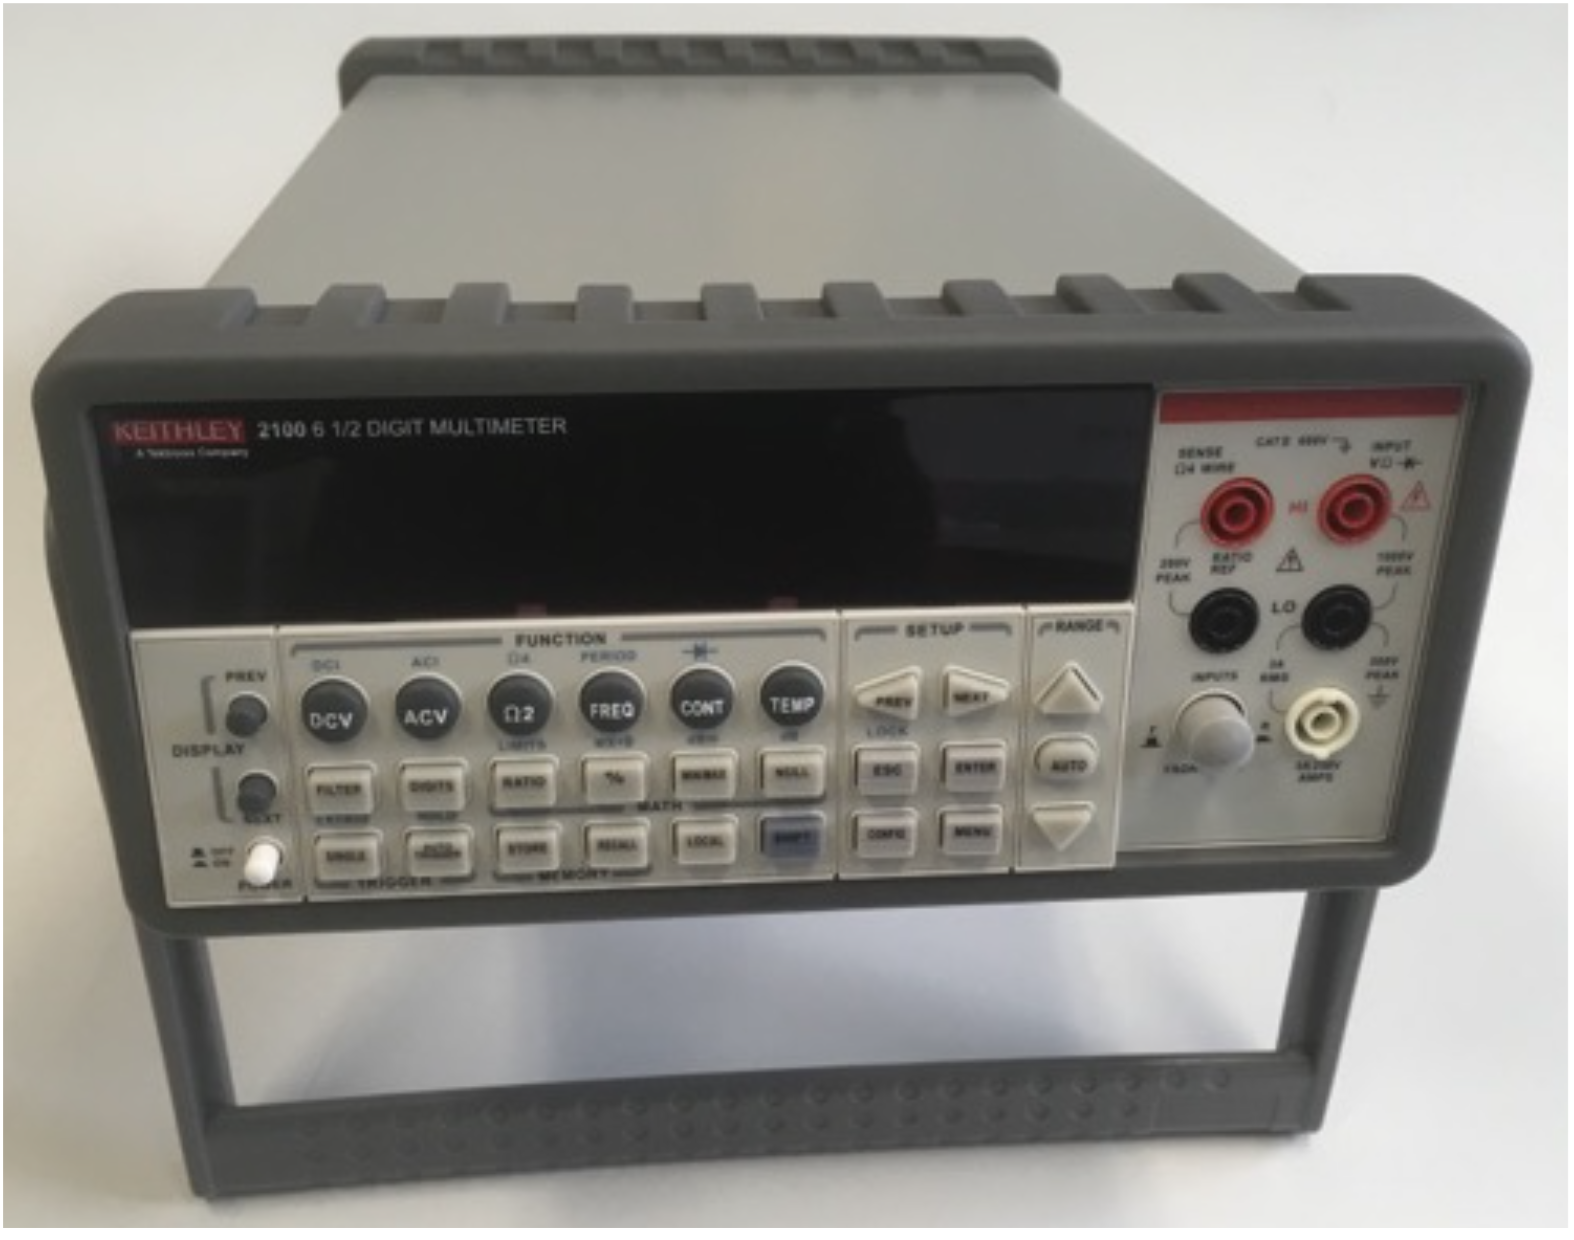
\includegraphics[width=14cm]{Figures/Keithlay.eps}
%\caption{.} 
%\label{fig:Keithlay} 
%\end{center}
%\end{figure}
%-------------------------------
\section{Calibration in End-station}
%-------------------------------
%\section{Gold standard}
%-------------------------------
%\section{Working standard}
\section{Summary}








 
% Chapter 1

\chapter{Beam position monitor} % Main chapter title

\label{Chapter6} % For referencing the chapter elsewhere, use \ref{Chapter1} 
One of the serious systematic error is beam position
We are developing Beam position monitor (BPM) for accurate measurement of beam position.
Previous study in LIGO have achieved 0.3~\% of uncertainty by using Telephoto camera system.
They place the telephoto camera at 8~m far from the ETM. On the other hand, That of KAGRA is 36 m where is 4.5 times larger. Therefore, one of the most difficult technologies of calibration is beam position measurement.

We will demonstrate the system of BMS as  the new technology. The BMS system is consists of XXXX parts as shown in Fig.XXXX.

According to Eq.(\ref{eq:dx}), vector $\vec{a}$ and $\vec{b}$ corresponds to the rotation effect. $\vec{a}$ can be written as
\begin{equation}
\vec{a}=\vec{a_1} + \vec{a_2},
\end{equation}
where $\vec{a_1}$ and $\vec{a_2}$ are position vectors of two Pcal beams. We can measure the beam position of main interferometer, $\vec{b}$, as well.
We can obtain the rotation term as
\begin{equation}
\frac{I}{M}\vec{a} \cdot \vec{b}
\end{equation}
,where $I$ and $M$ are inertial moment and mass of test mass.

Furthermore, the misaligned beam positions make the elastic deformation on the mirror surface due to asymmetry. It is one of the serious systematic errors.
Detail of the elastic deformation is described in Sec.~\ref{Chapter4}.

\section{Instlation}
The installation phase of beam position monitor consists of two phases.
In first phase, we place the TCam system at the side of EXA and EYA chamber.
Detail of TCam is described in XXX. We connect the TCam and control PC (Raspberry pi) and operate it.
The purpose of TCam is not only calibration work but also other application.
We will monitor the pollution of water due to cryo-pumping effect. The taken picture will be analyzed automatically.
In second phase, we place the QPD and the pico motor. We will control the beam position using these components.
\section{Operation}
All the system is operated by MEDM system as shown in Fig.XXX.
The operation strategy is listed as follows:
\begin{enumerate}
 \item Take a picture with illuminator. We set the integration time to 30 sec.
 \item Estimate the origin of mirror coordinate using edge shape of the mirror.
 \item Turn off the illuminator and take picture with 30 sec integration time.
  \item Estimate the Pcal beam position and main interferometer position with no illumination picture.
   \item Make a picture overplayed the coordinate of Pcal and origin as shown in Fig.XXXX.
\end{enumerate}
\section{Analysis}
\section{Demonstration test}
\section{Summary}

  
% Chapter 1

\chapter{Beam position monitor} % Main chapter title

\label{Chapter7} % For referencing the chapter elsewhere, use \ref{Chapter1} 
 
% Chapter 1

\chapter{Future upgrades} % Main chapter title

\label{Chapter7} % For referencing the chapter elsewhere, use \ref{Chapter1} 

\section{Photon stimulator}
We can apply the photon calibrator technologies for photon pressure actuator.
Then, we need to inject four laser at the node circle of the end test mass.

\section{Optical lever}
We place the QPDs on the receiver module. So, we can use the photon calibrator as displacement and angle sensing optical lever.
We expect to decouple the displacement and rotation effect by using two beams.
 

%----------------------------------------------------------------------------------------
%	THESIS CONTENT - APPENDICES
%----------------------------------------------------------------------------------------

%\appendix % Cue to tell LaTeX that the following "chapters" are Appendices

% Include the appendices of the thesis as separate files from the Appendices folder
% Uncomment the lines as you write the Appendices

%% Appendix A

\chapter{Propagation of calibration errors into the estimated source 
parameters}
\label{AppendixA}

In order to understand the propagation of systematic errors from calibration 
parameters to the estimated source parameters, a simple simulation is made 
as follows.

\section{DARM feedback loop modeling}

As discussed in Chapter~\ref{Chapter1}, the response function of 
interferometer system $R(f)$ can be written as 
\begin{equation}
R(f) = \frac{1+G(f)}{C(f)}
\end{equation}
where $G(f) = C(f)D(f)A(f)$ is the DARM open loop gain, $C(f)$ is the sensing 
function, $D(f)$ is the digital filters and $A(f)$ is the actuator function.
As a typical configuration, we used $G(f)$ and $A(f)$ based on the LIGO O1/O2 
configuration~\cite{LIGO-CAL,Tuyenbayev}. Fig.~\ref{fig:appa-olg} shows the 
transfer functions of open loop gain and actuators. Here we assume the 
three-stage pendulum and second and third stages contribute the control 
in the frequency range we are interested in. For the sensing function, 
in the case without Signal Recycling Cavity (SRC) detuning, $C(f)$ 
can be approximated by a single pole,
\begin{equation}
C(f)=\frac{G_c}{1+{\rm i}f/f_c},
\end{equation}

where $G_c$ is the optical gain, $f_c$ is the coupled cavity pole frequency.

In this simulation, we assume three parameters, $G_c$, $f_c$ and $A_T$ 
to be calibrated and tracked, where $A_T$ is the scale factor of 
the actuator function. Figs.~\ref{fig:appa-cal1},\ref{fig:appa-cal2} and
\ref{fig:appa-cal3} show the deformations 
of $R(f)$ due to the calibration bias on these three parameters.
These results agree with Ref~\cite{Tuyenbayev}. Since the assumed 
transfer functions are not exactly the same as Ref~\cite{Tuyenbayev} 
there are minor differences.

\begin{figure}
\begin{center}
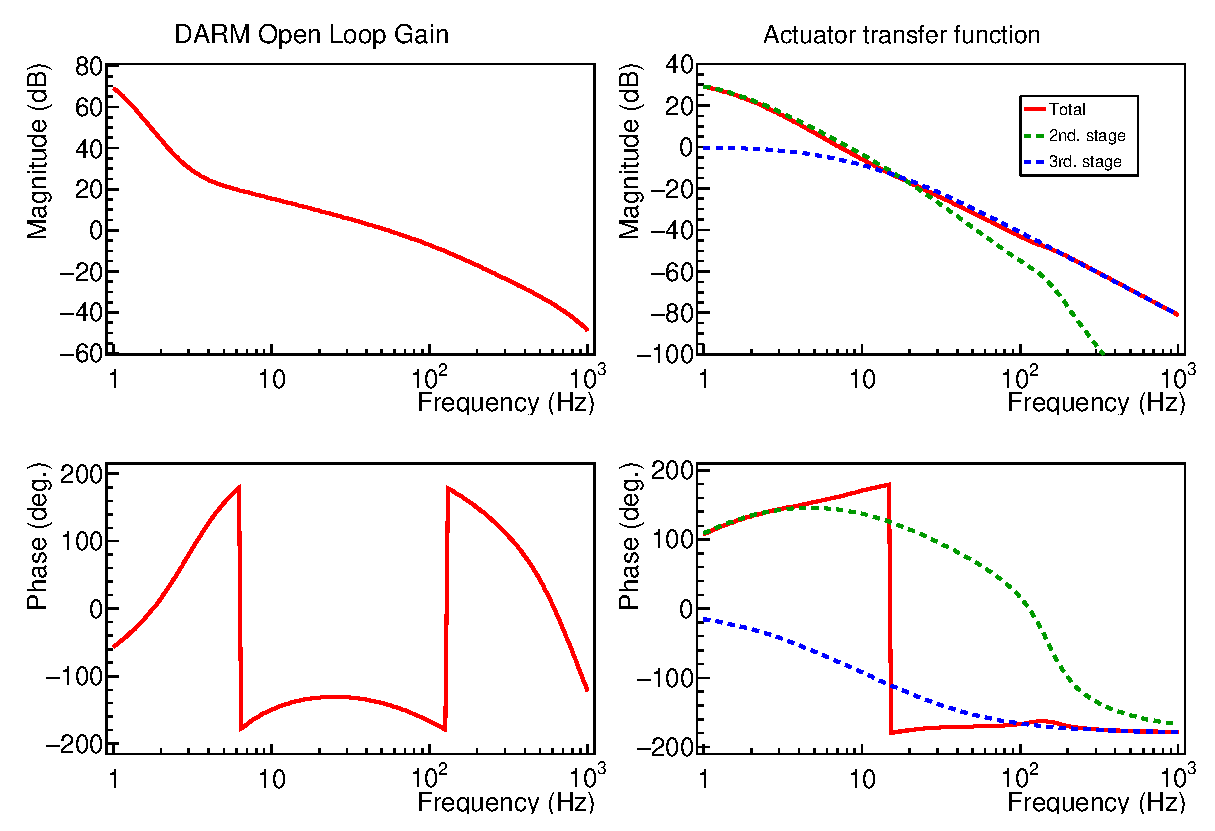
\includegraphics[width=\linewidth]{Figures/appa-olg.eps}
\caption{Transfer functions of DARM open loop gain and actuators assumed in 
this simulation.}
\label{fig:appa-olg} 
\end{center}
\end{figure}

\begin{figure}
\begin{center}
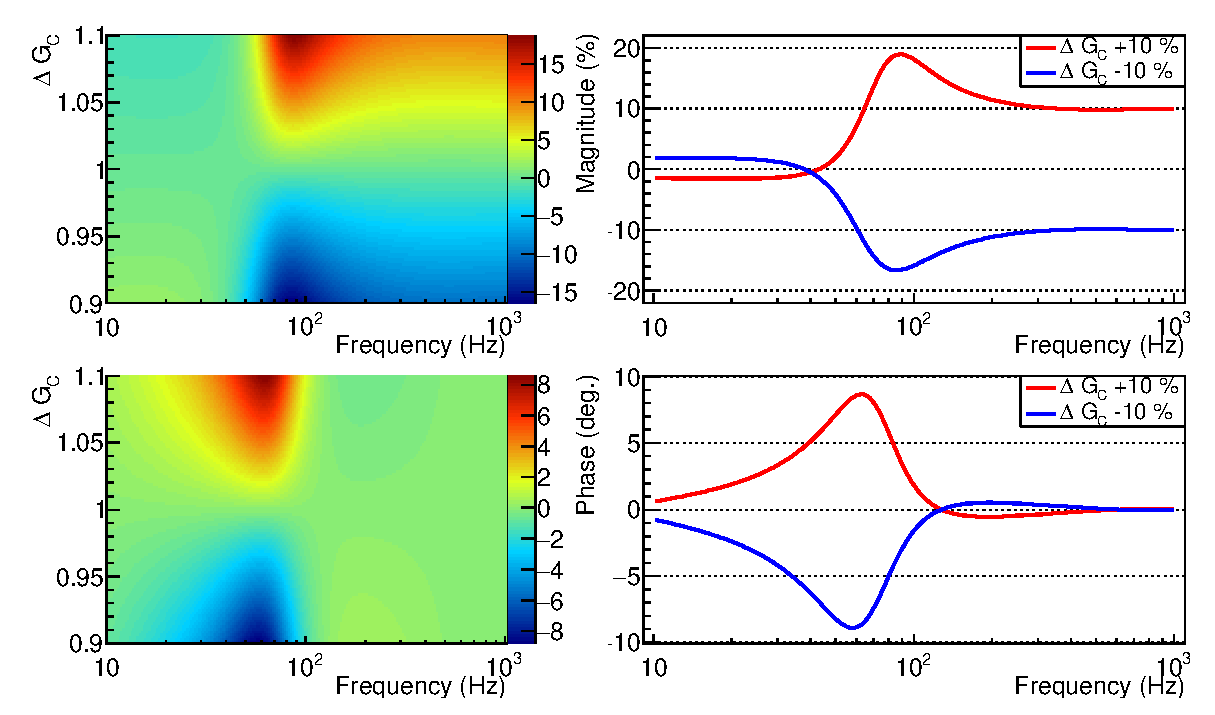
\includegraphics[width=\linewidth]{Figures/appa-cal1.eps}
\caption{Deformation of $R(f)$ due to the relative calibration bias on $G_C$.}
\label{fig:appa-cal1} 
\end{center}
\end{figure}

\begin{figure}
\begin{center}
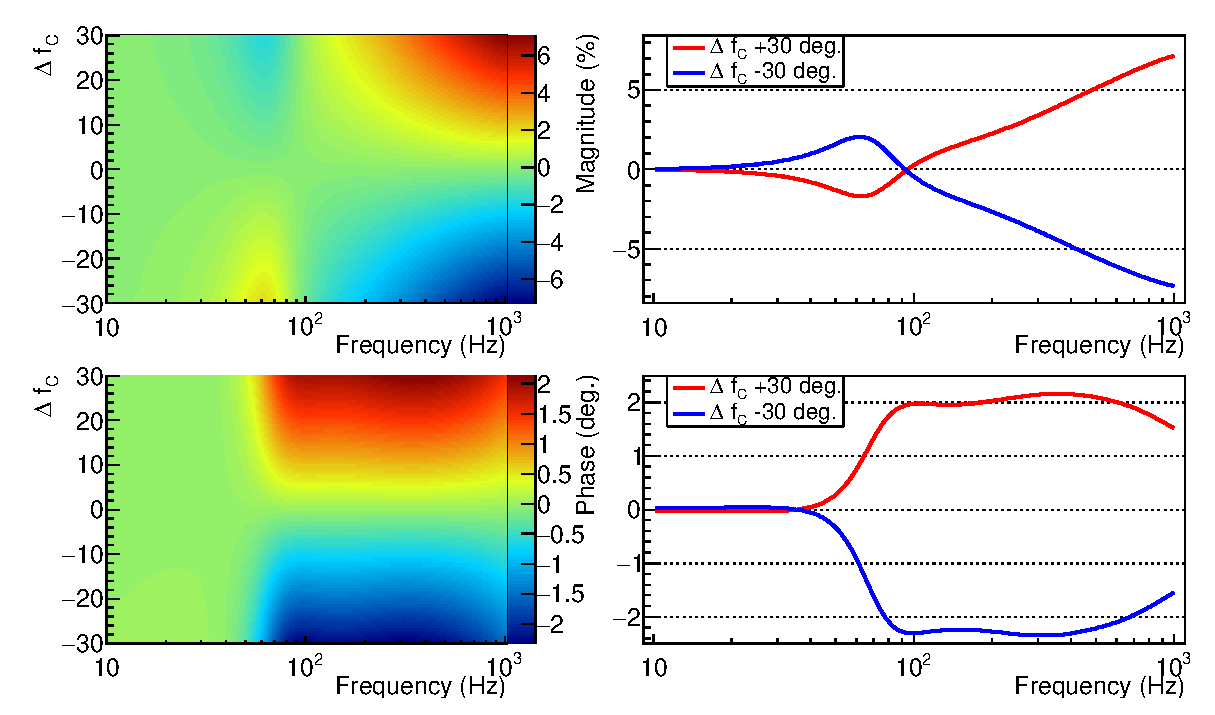
\includegraphics[width=\linewidth]{Figures/appa-cal2.eps}
\caption{Deformation of $R(f)$ due to the relative calibration bias on $f_C$.}
\label{fig:appa-cal2} 
\end{center}
\end{figure}

\begin{figure}
\begin{center}
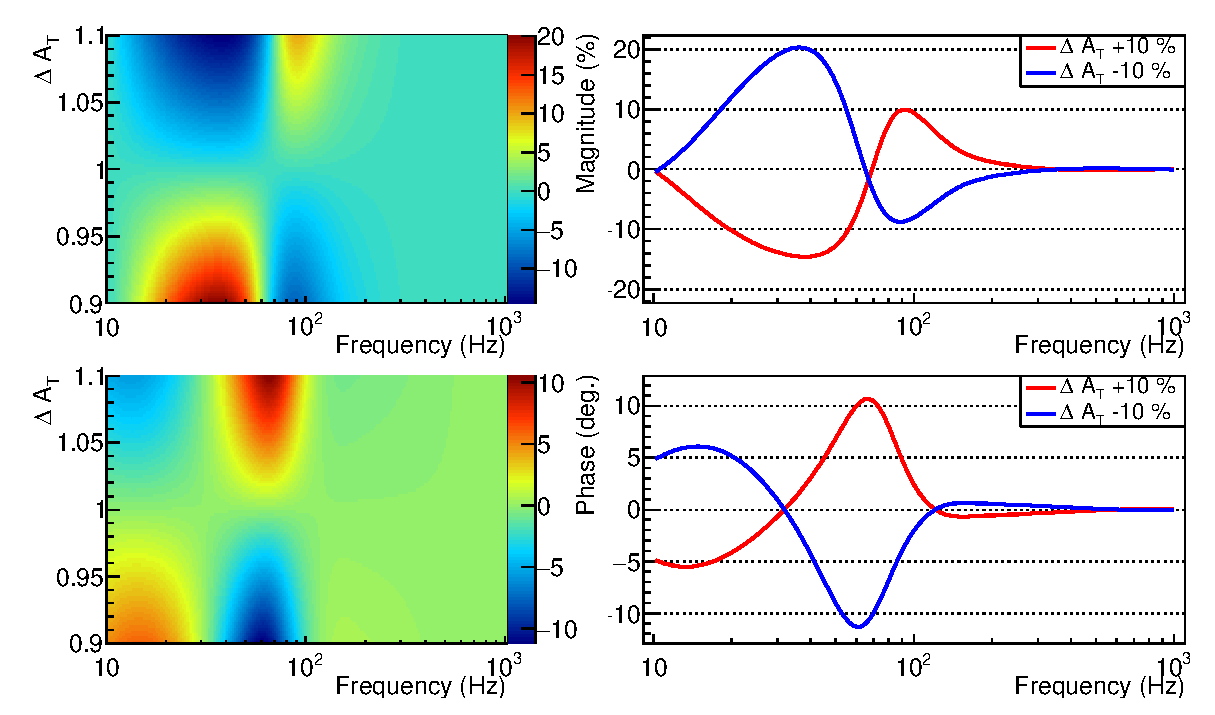
\includegraphics[width=\linewidth]{Figures/appa-cal3.eps}
\caption{Deformation of $R(f)$ due to the calibration bias on $A_T$.}
\label{fig:appa-cal3} 
\end{center}
\end{figure}

\newpage
\section{Waveform modeling}
As a simple example, we assume the GW signal in the frequency domain from 
the compact binary coalescence by using the second order post-Newtonian (2-pN) 
formalism and ignoring any effects due to the spins with five free parameters, 
a total system mass, $M=m_1+m_2$,
a symmetric mass ratio $\eta=m_1 m_2/M^2$, the source distance, $D$, 
a coalescence time $t_c$, and a coalescence phase $\phi$,
\begin{equation}
h(f) = \frac{1}{2\pi^{2/3}c^{3/2}}\frac{(GM)^{5/6}}{D}\left(\frac{5\eta}{6}\right)^{1/2}f^{-7/6} e^{i(2\pi ft_c+\phi+\Psi(f))},
\end{equation}
where 
\begin{equation}
\Psi(f)=\sum_{i=1}^4 a_i \xi_i(f),
\end{equation}
\begin{equation}
a_1=\frac{3}{128\eta}q^{-5/3},
\end{equation}
\begin{equation}
a_2=\frac{1}{384\eta}\left(\frac{3\:715}{84}+55\eta\right)q^{-1},
\end{equation}
\begin{equation}
a_3=-\frac{1}{128\eta}48\pi q^{-2/3},
\end{equation}
\begin{equation}
a_4=\frac{3}{128\eta}\left(\frac{15\:293\:365}{508\:032}+
\frac{27\:145}{504}\eta+\frac{3\:085}{72}\eta^2\right)q^{-1/3},
\end{equation}
$\xi_1(f)=f^{-5/3}$, $\xi_2(f)=f^{-1}$, $\xi_3(f)=f^{-2/3}$, 
$\xi_4(f)=f^{-1/3}$, and $q=\pi GMc^{-3}$~\cite{Tanaka-Tagoshi}.

The parameters estimation is done with the maximum likelihood method, 
\begin{equation}
{\rm ln}L = -\frac{1}{2}\int_{f_{min}}^{f_{max}}df\frac{|d(f)-h(f)|^{2}}{S(f)},
\end{equation}
where $f_{min}$ and $f_{max}$ are the filtered frequency range, 
$d(f)$ and $h(f)$ are observed and estimated wave forms, and 
$S(f)$ is the power spectrum density of the detector noise.

In this analysis we assume the source parameters similar to GW150914 
and fittin between 30 and 300~Hz.
Fig.~\ref{fig:appa-cmp} shows the comparisons of relative deformed and fitted 
wave forms with respect to the true one. Finaly, we estimated the bias on 
the five source parameters. Left part of Fig.~\ref{fig:appa-sim} shows 
the systematic bias on the five source parameters, while rigt part of 
Fig.~\ref{fig:appa-sim} shows the extreme case where the source distance is 
200~Mpc away and the signal-to-noise ratio is high enough.

\begin{figure}
\begin{center}
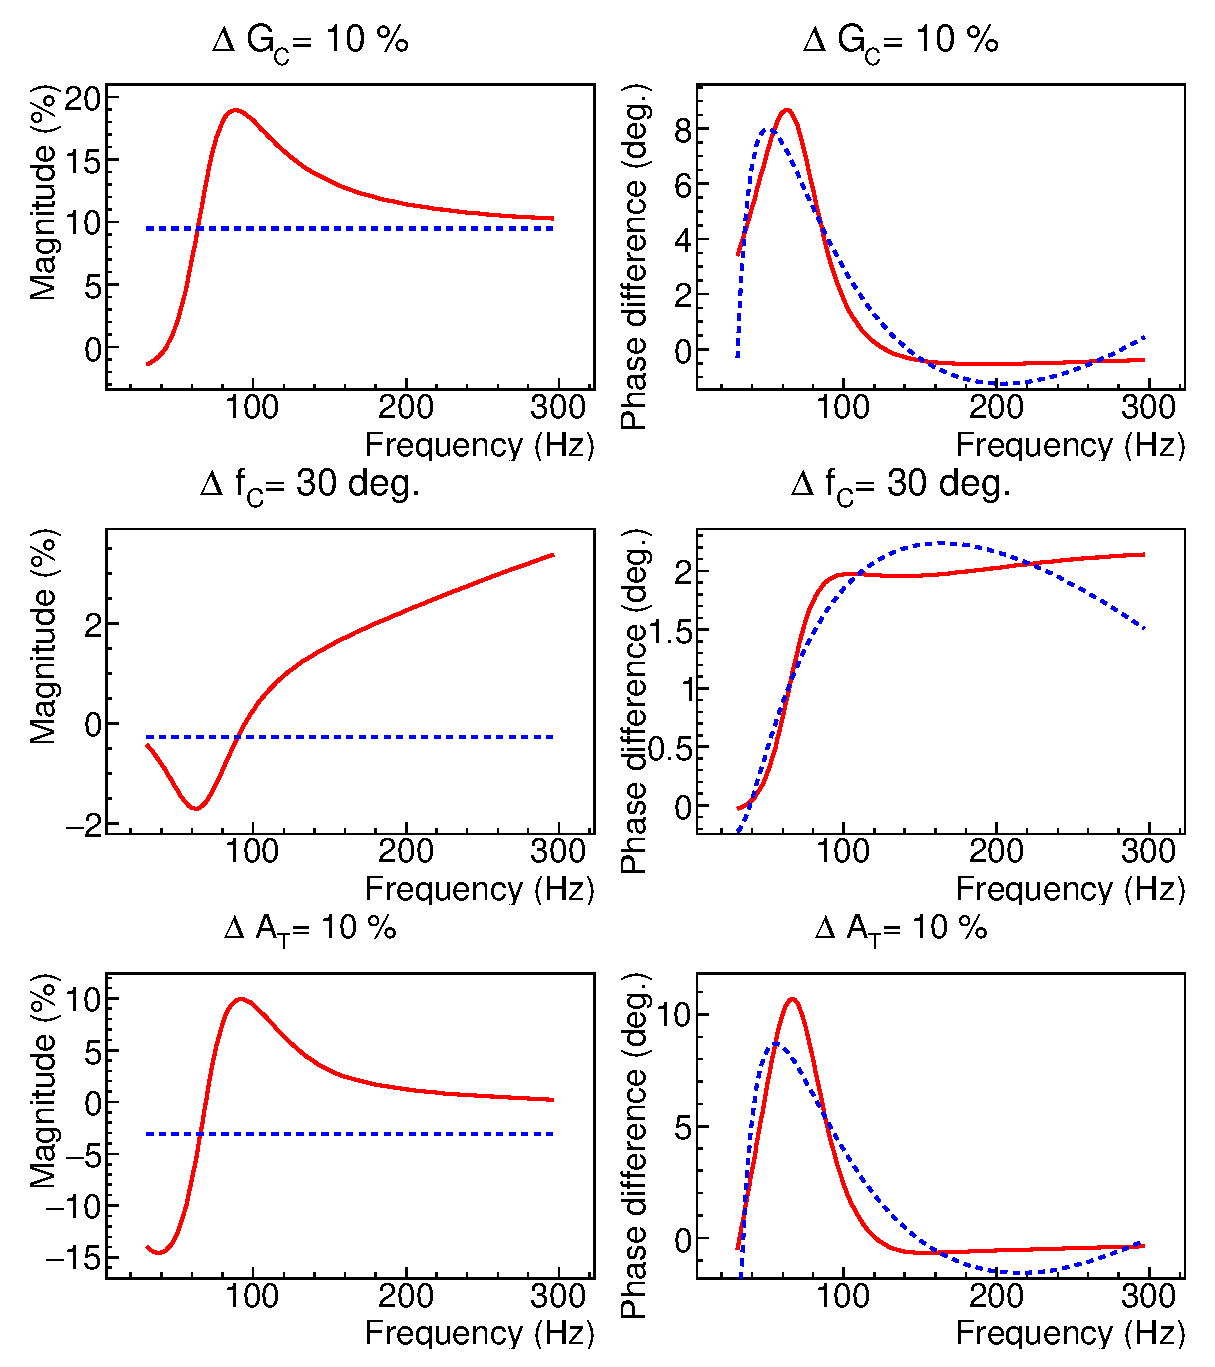
\includegraphics[width=\linewidth]{Figures/appa-cmp.eps}
\caption{Comparisons of relative deformed (red solid lines) and fitted 
(blue dashed lines) wave forms with respect to the true one, 
in the three cases where $G_C$, $f_C$ and $A_T$ are biased by 
$\pm 10\%$, $\pm 30$ deg., and $\pm 10\%$, respectively.}
\label{fig:appa-cmp} 
\end{center}
\end{figure}

\begin{figure}
\begin{center}
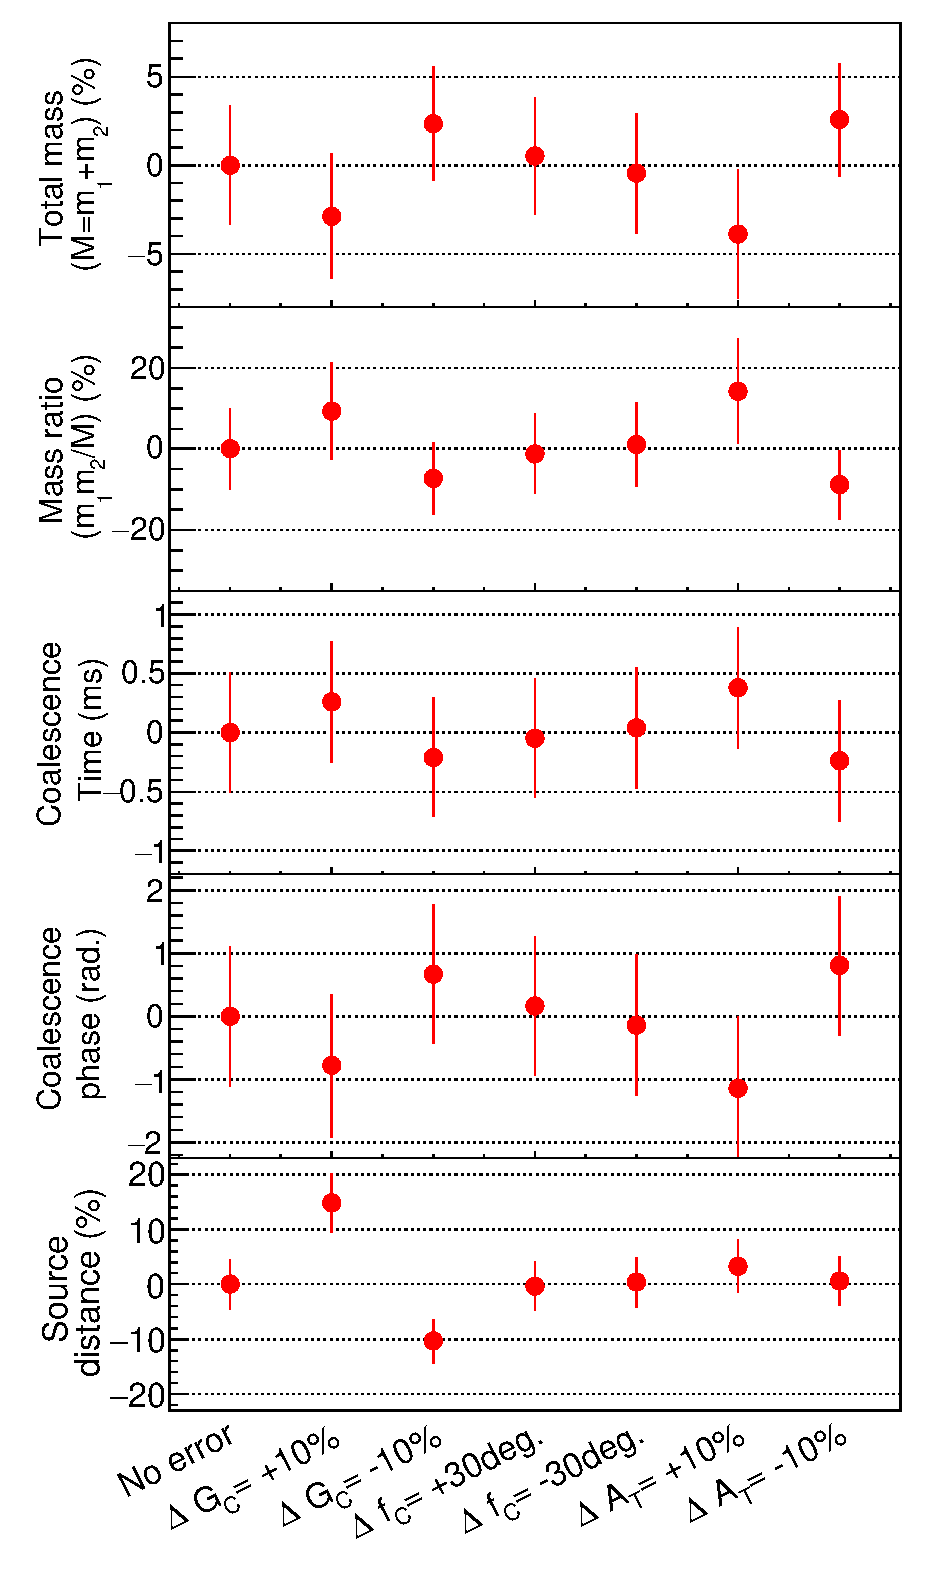
\includegraphics[width=0.49\linewidth]{Figures/appa-sim1.eps}
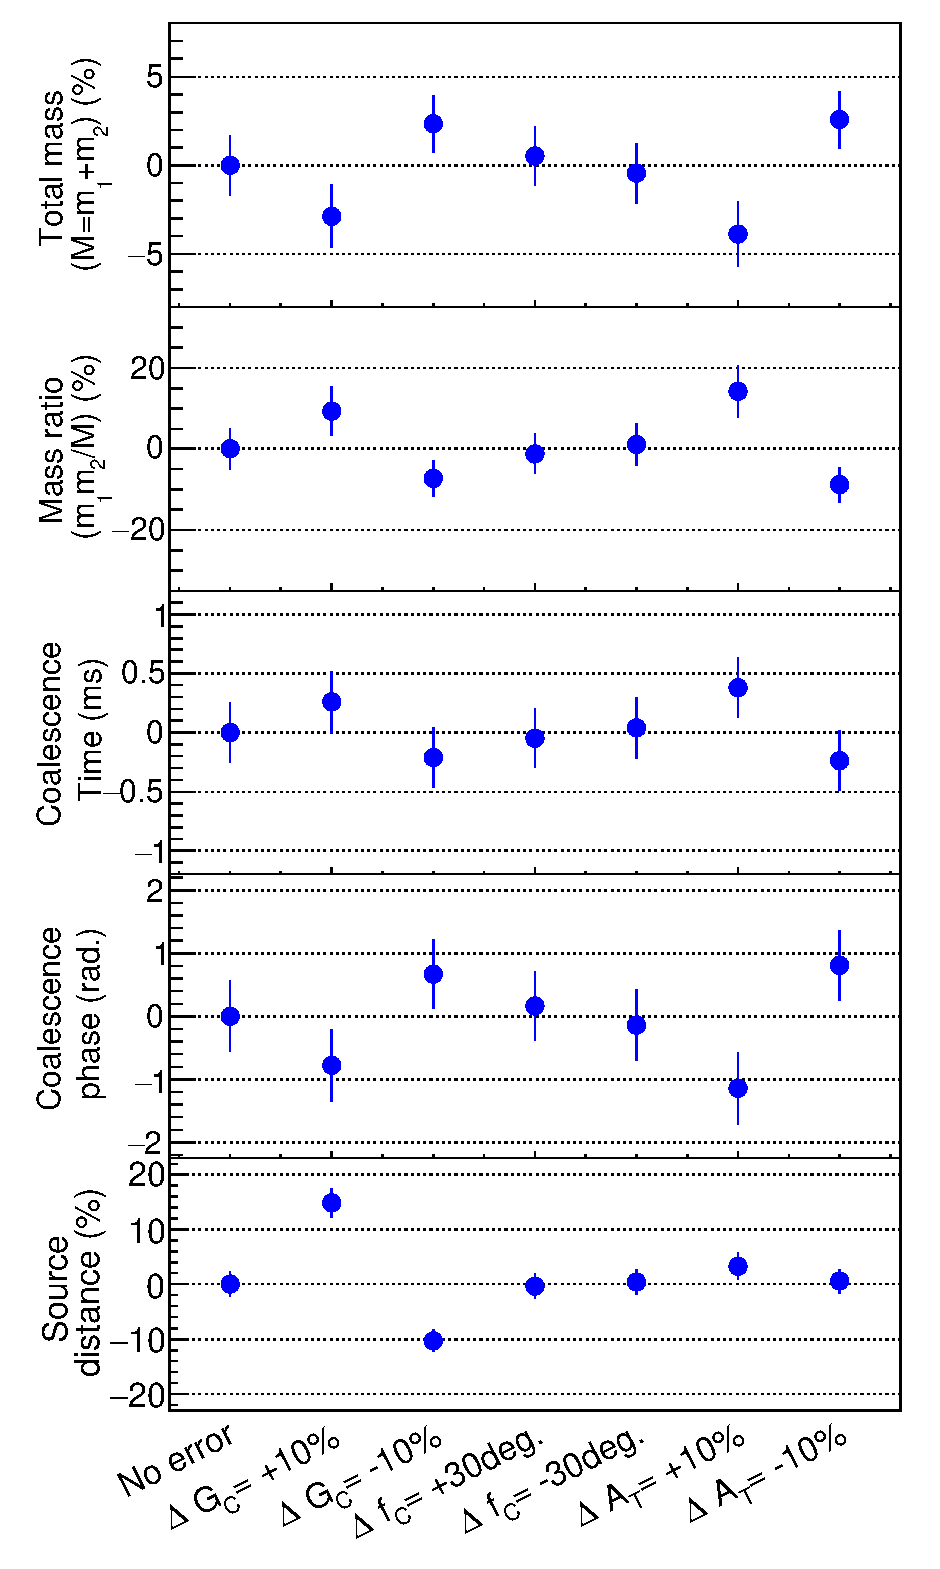
\includegraphics[width=0.49\linewidth]{Figures/appa-sim2.eps}
\caption{The systematic bias on the five source parameters as a 
function of variations of calibration parameters assuming the 
signal similar to GW150914 (left), and the extreme case where 
the GW150914 source is 200~Mpc away (right).}
\label{fig:appa-sim} 
\end{center}
\end{figure}

%\include{Appendices/AppendixB}
%\include{Appendices/AppendixC}

%----------------------------------------------------------------------------------------
%	BIBLIOGRAPHY
%----------------------------------------------------------------------------------------

\printbibliography[heading=bibintoc]

%----------------------------------------------------------------------------------------

\end{document}  
